\documentclass[
  hyper,    
  lang=cn,
  class=book,
  bib_index={load},
  mathSpec={envStyle=leftbar, alias},
  toc={column=2, title=目录},
]{zlatex}
% packages
\usepackage{expl3}
\usepackage{xfp}
\usepackage{zhnumber}
\usepackage{pdfpages}
\usepackage{booktabs}
\usepackage{longtable}
\usepackage{verbatim}
\usepackage{pifont}
\usepackage{multicol}
\usepackage{framed}
\usepackage[bottom]{footmisc}
\usepackage{xltxtra} 
\usepackage{indextools}


% Set up
\zlatexColorSetup{ definition  = blue }
\indexsetup{level=\chapter}
\makeindex[title=部分命令/名词索引, columns=2]
\let\cmd\zlatexVerb
\newcommand{\Footnote}[1]{\stepcounter{footnote}\footnote[\thefootnote]{#1}}
\zlatexFramed{leftbar}[gray]
\newcommand{\zkey}[1]{\texttt{<#1>}}
\def\mstyle#1{\noindent\lower.25ex\hbox{\ding{224}}\;\textbf{#1}\par}
\usepackage{minted}
\definecolor{bg}{rgb}{0.95,0.95,0.95}
\setminted{
  fontsize=\small,
  bgcolor=bg, 
  breaklines=true, 
  tabsize=2,
  breakanywhere=true,
  breakanywheresymbolpre=,
  breaksymbolleft=,
}


% ----------------------------------------------------------------------
%  for special reasons, change the module loading function temporarily
% ----------------------------------------------------------------------
\usepackage{ztikz}
\usetikzlibrary{calc}
\ExplSyntaxOn
\cs_set_nopar:Npn \g__ztikz_load_module:n #1 {
  \clist_map_inline:nn {#1} {
    \file_if_exist_input:nF {ztikzmodule.##1.tex} {
      \msg_new:nnn {ztikz} {module-not-found} {Module~`##1'~not~found.}
      \msg_error:nnn {ztikz} {module-not-found} {##1}
    }
  }
}
\ExplSyntaxOff
\ztikzLoadModule{cache, wolfram, python, gnuplot, zdraw}



\title{zTikZ manual}
\author{Eureka}
\date{\today}
\begin{document}
\maketitle
\frontmatter
\tableofcontents
\mainmatter
\part{Document}
% ----------------------------------------------------------------------
%                              ztik doc
% ----------------------------------------------------------------------
\chapter{zTikZ{}宏包}\label{start-use-package}
目前zTikZ宏包能够在Linux/Windows下编译运行,在MacOS上进行了部分的测试,部分功能不能使用.
详细的测试信息或者是兼容情况请参见后续 Set Up 章节. 目前本宏包主要包含如下几个模块:

\begin{itemize}
  \item gnuplot: 调用外部程序 gnuplot 进行图形的绘制
  \item wolfram: 调用 mathematica 或者是 wolframscript 进行计算
  \item python: 调用 python 进行计算,绘图以及表格等操作
  \item zdraw: 目前本模块还处于测试阶段,但是目前基于 l3draw 已经能够完成基本图形的绘制
  \item cache: 本模块用于缓存计算结果,减少重复计算的时间. 可以应用于上述的 wolfram, python 模块
\end{itemize}

默认情况下不会加载以上的任意一个模块,在 ztikz 宏包中仅包含用于绘制点,直线,坐标轴和基本多边形的命令.
想要使用上述的模块也很简单,在导言区使用如下命令进行加载:
\begin{minted}{latex}
\ztikzLoadModule{cache, gnuplot}
\end{minted}

上述命令就表示加载 cache 和 gnuplot 模块. 一个值得注意的事情:只有你加载对应的 module 时,对一个的
脚本文件才会被写入项目文件夹下.

\section{基本介绍}
\subsection{开发背景}
其实还有很多基于 TikZ 并且提供和 zTikZ 宏包中绘图功能差不多宏包,这其中就有:
\begin{itemize}
    \item 一个TiKZ的常见命令封装:\href{https://ctan.org/tex-archive/graphics/pgf/contrib/tzplot}{tzplot}
    \item 一个3D绘图的TiKZ库:\href{https://ctan.org/pkg/tikz-3dplot}{tikz-3dplot}
    \item 一个基于 PSTricks 的函数绘图包:\href{https://ctan.org/pkg/pst-func}{pst-func},可以用于绘制部分的特殊函数
\end{itemize}

用户如果觉得 zTikZ 库并不符合你的胃口,不妨试试上面的几个宏包,或者是直接使用原始的 pgf/tikz 命令进行绘图.
和 TikZ 相关的网站也是十分丰富的,以下推荐一个TikZ绘图的网站:\href{https://texample.net/tikz/examples/}{TikZ Example}.
这个网站中有着丰富的绘制样例并且提供了对应的绘图代码.

\subsection{zTikZ{}功能}
zTikZ宏包主要用于绘图与计算, 其中的绘图功能支持\cmd{python, mathematica, gnuplot}, 但是
这并不意味着你需要安装以上给的所有软件,每一个软件(模块)之间是独立的.你需要什么功能的,你就在
操作系统上安装对应的模块.

zTikZ主要提供两个大功能: \textbf{绘图, 计算}.
绘图部分包括 TikZ 自身的绘图功能(2d部分)\Footnote{由于3d绘图部分涉及的几个变换矩阵接口我还没想好怎么在 zTikZ 中声明, 
所以目前 zTikZ 不提供3d绘图功能},python 的 matplotlib 绘图,以及 mathematica 代码绘图. 计算部分
包括\LaTeX3的 {xfp} 宏包模块,python 的 sympy 计算模块,以及 mathematica 模块. 

\begin{remark}
zTikZ 未来不会支持 3d 绘图部分了, 如果用于想要使用这一方面的功能,还请使用其余的宏包或者使用其他的专业软件.
这里推荐使用 Asymptote.
\end{remark}

\subsection{缓存机制}
zTikZ除了提供必要的和外部程序互动的功能外,还内置了一套 cache 系统,zTikZ 会自动把\TeX{}和
外部程序交互产生的结果缓存下来,并且记录下\LaTeX{}文档中调用部分源代码的 Hash 值. 如果\LaTeX{}文档中的源代码
Hash值改变,那么 zTikZ 就会重新和外部程序交互,重新产生结果,并且缓存新的 Hash 值.如果文档中的
源代码的Hash值没有变,那么 zTikZ 就会直接调用上一次的缓存结果. 这样做的好处是显而易见的,就是
我们不必反复的编译没有变化的内容,直接引用缓存,大大的减少了编译的时间. 

目前zTikZ中的所有模块:TikZ/gnuplot\Footnote{\cmd{tikzpicture}环境或者是\cmd{\tikz}命令生成图片的 cache 机制是依靠
tikz的\cmd{external}库实现的,感兴趣的可以去看看}, Python/sympy, Python/matplotlib, Mathematica 都已经实现
了缓存机制. 在实际测试中,在结果缓存后,再次编译源文档的时间和直接插入对应数量的图片的时间几乎一致.如果你不想使用缓存机制,那么可以
不加载\cmd{cache} 模块.

\begin{remark}Known Bugs:\par
\mstyle{Hash Recover}
如果一个环境最开始的Hash值为``A'', 在你修改了这个环境的内容后,使得此环境中
代码的Hash值变为 ``B''. 但是如果你现在再次修改会Hash值为 ``A''时对应的源代码,此刻的Hash值已经缓存在了
\cmd{ztikz.hash} 中,所以再次编译时此环境对应的绘制结果并不会改变.仍然为Hash值为``B''时的结果. 

\mstyle{Conflict to indextool}
有可能你在启用缓存模块后,发现编译报错 \texttt{missing \textbackslash begin\{document\}...}. 这个问题和宏包 indextool 的索引
功能有关. 可以尝试先注释 \cmd{\makeindex, \printindex} 命令,在图片缓存结束后,取消注释,然后再生成索引.
\end{remark}

\section{Set Up zTikZ}
\subsection{兼容情况}
目前\cmd{zTikZ}模块已经可以在 Windows 和 Linux 下正常运行, 各个平台兼容性如下:

\hspace*{10em}\parbox{8cm}{
\begin{itemize}
  \item Windows: \TeX{}Live最低版本2023
  \item Linux: \TeX{}Live最低版本2022
  \item MacOS: Mac\TeX{}由于缺少 {l3sys-shell} 宏包(或者不适配),所以并不兼容
\end{itemize}}

在Linux平台上并没有什么需要注意的事项,重点是Windows平台上的兼容性; 要使得 {zTikZ}正常运行,
那么在引用对应的模块后,对应的系统中(默认添加了环境变量)须有对应的软件.以下是部分的软件配置事项:
\begin{itemize}
  \item {sed}: 模块 gnuplot, python 中部分命令基于绘图脚本中的函数以及绘制样式替换,目前采用sed实现,
    后续可能会考虑去除 {sed}依赖.
  \item {python}: 用于运行python脚本进行符号计算与绘图,需要Python库 {sympy, scipy}.
  \item {wolframscript}(可选):如果需要使用 wolfram 模块的功能,那么需要安装WolframScript或
      对应软件Mathematica.执行命令时可以选择在云端执行,这样就避免调用本地Mathematica计算内核. 
\end{itemize}

\subsection{环境配置}
\subsubsection{Linux}
在Linux下除了wolfram应该都是很好安装的, 直接使用Linux发行版自带的包管理器即可.在这里我提供一个在
WSL中使用Windows下Mathematica 的方法. 其实就是在Linux下创建一个从Linux到Windows的软连接,如下:

\begin{minted}{shell}
ln -sf "/mnt/c/Program Files/Wolfram Research/WolframScript/wolframscript.exe" /usr/bin/wolframscript    
\end{minted}

具体的wolframscript的路径根据实际情况而定.

\subsubsection{Windows}
因会使用到 {gnuplot},所以在 Windows下需要在系统环境变量中添加 {gnuplot} 的路径.并且
在编译此文档时需要加上对应的 \cmd{--shell-esape}参数;在Windows平台,由于\TeX{}Live的编译配置,
需确保系统环境变量\cmd{PATHEXT}中已经删除\cmd{.PY}后缀. zTiKZ在Windows下的适配是没有Linux下那么好的,
建议在Linux下使用本宏包.\Footnote{zTiKZ中的Wolfram模块可以在Windwos上使用并且可以输入\texttt{\textbackslash, \#, \$}等特殊字符
,这一点弥补了 \href{https://github.com/stevenliuyi/latex-alpha2}{latexalpha2} 的不足}.

\subsubsection{MacOS}
在MacOS下由于缺少 {l3sys-shell}宏包(或者是不适配),所以并不兼容.后续我可能会考虑重 zTikZ 中用到的
部分 {l3sys-shell}宏包中的命令,如果此需求比较大的话.当然,欢迎各位提 PR, 一起完善这个宏包.

\section{绘图功能}
\subsection{Builtin TikZ}
zTikZ目前的绘图逻辑为:
\begin{itemize}
    \item 通过sed修改脚本中的函数或定义域范围
    \item 通过\cmd{write18}调用gnuplot运行修改后的脚本
    \item 然后使用命令\cmd{\draw[<style>] plot file {<data>};} 绘制生成的数据文件
\end{itemize}

但是TikZ内部已经提供了直接调用gnuplot程序的命令,格式如下:
\begin{minted}{latex}
\draw[<draw style>] plot[<id>] function{<function>};
\end{minted}

当指定内置命令中为\cmd{<id>}时,在\cmd{<name>.tex} 文件的根路径下会产生两个文件;第一个是、
gnuplot绘制的样式文件\cmd{<name>.<id>.gnuplot},第二个是gnuplot产生的数据文件\cmd{<name>.<id>.table}.
其中的\cmd{<function>}可用值可以参见\cref{tab:gnuplot-functions}. 

内置的命令也支持另外两种格式: {parametric, raw gnuplot}. 第一个表示绘制参数方程,第二个表示直接
在文档中输入gnuplot绘图代码. 两者的基本格式如下:
\begin{minted}{latex}
% 启用参数方程绘制,默认变量为 t
\draw[<draw style>] plot[parametric, <id>] function{<function (t)>};

% 启用直接输入gnuplot代码绘制
\draw[<draw style>] plot[<id>] function{set samples 25; plot sin(x)};
\end{minted}

目前为了几个绘图命令的统一,zTikZ并没有采用内置的这一命令,而是直接调用了另一个外部程序sed用于辅助.
在后续去除sed依赖时可能会考虑重写这一部分命令.但是,并不会改变已有的命令接口. 在这里给出一个
这些内置命令的绘图样例:

\begin{figure}[!htb]
    \centering
    \begin{tikzpicture}[domain=0:4]
    \draw[very thin,color=gray] (-0.1,-1.1) grid (3.9,3.9);
    \draw[->] (-0.2,0) -- (4.2,0) node[right] {$x$};
    \draw[->] (0,-1.2) -- (0,4.2) node[above] {$f(x)$};
    \draw[color=red] plot[id=x] function{x} node[right] {$f(x) =x$};
    \draw[color=blue] plot[id=sin] function{sin(x)} node[right] {$f(x) = \sin x$};
    \draw[color=orange] plot[id=exp] function{0.05*exp(x)} node[right] {$f(x) = \frac{1}{20} \mathrm e^x$};
\end{tikzpicture}
    \caption{12 Using Built-in TikZ Function}
    \label{fig:12-inverse-function-2}
\end{figure}

\inputminted{latex}{./example_12.tex}

后续的统计图绘制命令也是继承自TikZ中内建的命令,比如后续的\cmd{\BarPlot}命令是如下内建命令的缩写:
\begin{minted}{latex}
\draw[<style>] plot[ycomb, <other style>] file{<data>};
\end{minted}

更多的关于TikZ中这几个原生命令的使用方法请参见附录:\cref{chap:tikz_function_plot} 中TikZ官方文档中截取的说明.

\subsection{gnuplot}
zTikZ提供了绘制绝大部分函数的命令,同时zTikZ的命令可以和 {tikz} 中的命令``融合'',它们
可以在同一个 {tikzpicture} 环境中使用. 而且,zTikZ对函数绘制时的坐标进行了``对齐''. 
也就是zTikZ中命令的坐标,和 {TiKZ}中的命令的坐标, Geogebra中的坐标是一致的. 

为何要在zTiKZ中把坐标``对齐''? 试想这么一个情景:你在Geogebra中找到了两个函数图像的交点为 $P(1, 2)$,
首先使用TiKZ自带的\cmd{\filldraw}命令把 $P$点绘制出来, 然后使用zTikZ中
\cmd{\ShowPoint}命令再次绘制这个 $P$点. 然而结果就是:这两个 $P$点没有重合,尽管我们指定的坐标
都是 $(1, 2)$ -- 这就是为什么zTikZ要把坐标``对齐''. 这样还有一个好处,当你不方便使用 zTikZ 
求解某些特殊的点时,你可以在诸如 Geobebra 这样的软件中把对应的 $P$点求解出来,然后直接在zTikZ中
使用\cmd{\ShowPoint}命令绘制此点, 不用担心它们的坐标对齐.

在平面图形绘制方面,zTikZ提供了绘制函数命令,一些和坐标轴有关的命令以及部分的欧几里得几何相关的命令,
各命令\Footnote{zTiKZ中的命令基本上都遵守了Mathematica中的函数的命名规范}的名称如下:

首先是和坐标系统相关的部分命令:包括点,线,面和规则多边形的绘制以及交点的求解与绘制.
\begin{itemize}
    \item \cmd{\ShowPoint}\index{\cmd{\ShowPoint}}: 绘制点
    \item \cmd{\Polygon}\index{\cmd{\Polygon}}: 绘制正多边形
    \item \cmd{\ShowGrid}\index{\cmd{\ShowGrid}}: 绘制网格 
    \item \cmd{\ShowAxis}\index{\cmd{\ShowAxis}}: 绘制坐标轴
    \item \cmd{\ShowIntersection}\index{\cmd{\ShowIntersection}}: 绘制交点
    \item \cmd{\gnudata}\index{\cmd{\gnudata}}:引用gnuplot数据
\end{itemize}

其次,gnuplot 模块提供了如下和函数相关的绘制命令,包括常见的几种二维函数绘制以及普通的形如 $z=f(x,y)$ 形式的
三维函数的绘制:
\begin{itemize}
  \item \cmd{\Plot}\index{\cmd{\Plot}}: 绘制函数
  \item \cmd{\ParamPlot}\index{\cmd{\ParamPlot}}: 绘制参数方程
  \item \cmd{\ContourPlot}\index{\cmd{\ContourPlot}}: 绘制等高线图
  \item \cmd{\PolarPlot}\index{\cmd{\PolarPlot}}: 绘制极坐标图
  \item \cmd{\ListPlot}\index{\cmd{\ListPlot}}: 绘制散点图,只需要指定绘制参数中\cmd{opacity=0}
  \item \cmd{\StairsPlot}\index{\cmd{\StairsPlot}}: 绘制阶梯图
  \item \cmd{\StemPlot}\index{\cmd{\StemPlot}}: 绘制火柴棒图
  \item \cmd{\BarPlot}\index{\cmd{\BarPlot}}: 绘制条形图
  \item \cmd{\ShadePlot}(deprecated)\index{\cmd{\ShadePlot}}: 绘制渐变曲线(直线)
  \item \cmd{\Plotz}\index{\cmd{\Plotz}}: 绘制函数曲线 $z=f(x, y)$
            \item \cmd{\PlotPrecise}\index{\cmd{\PlotPrecise}}: 函数绘制精度
            \item \cmd{\PlotPrecise}\index{\cmd{\PlotPrecise}}: 函数绘制精度
  \item \cmd{\PlotPrecise}\index{\cmd{\PlotPrecise}}: 函数绘制精度
\end{itemize}


\begin{remark}
上述的\cmd{\StairsPlot, \StemPlot, \BarPlot, \ShadePlot}在绘制时只能够传入具体的数据文件,而非对应的方程.
\end{remark}

\subsection{Support Functions}
在开始介绍之前,我想先介绍一下gnuplot中内建的函数,见\cref{tab:gnuplot-functions},
摘录自: \href{http://www.bersch.net/gnuplot-doc/expressions.html#expressions-functions-floor}{gnuplot support functions}.

\begin{leftbar}
    Arguments to math functions in gnuplot can be integer, real, or complex unless otherwise noted.
    Functions that accept or return angles (e.g. sin(x)) treat angle values as radians, but this may 
    be changed to degrees using the command set angles.
\end{leftbar}

\begin{center}
    \begin{longtable}{lll}
        \caption{\textbf{Math library functions}}\\
        \toprule
        \textbf{Function} & \textbf{Arguments} & \textbf{Returns} \\
        \midrule
        \(\text{abs}(x)\) & any & $|x|$, absolute value of $x$; same type \\
        \(\text{abs}(x)\) & complex & length of $x$, $\sqrt{\text{Re}(x)^2 + \text{Im}(x)^2}$ \\
        \(\text{acos}(x)\) & any & $\cos^{-1} x$ (inverse cosine) \\
        \(\text{acosh}(x)\) & any & $\cosh^{-1} x$ (inverse hyperbolic cosine) in radians \\
        \(\text{airy}(x)\) & any & Airy function $\text{Ai}(x)$ \\
        \(\text{arg}(x)\) & complex & the phase of $x$ \\
        \(\text{asin}(x)\) & any & $\sin^{-1} x$ (inverse sine) \\
        \(\text{asinh}(x)\) & any & $\sinh^{-1} x$ (inverse hyperbolic sine) in radians \\
        \(\text{atan}(x)\) & any & $\tan^{-1} x$ (inverse tangent) \\
        \(\text{atan2}(y,x)\) & int or real & $\tan^{-1}(y/x)$ (inverse tangent) \\
        \(\text{atanh}(x)\) & any & $\tanh^{-1} x$ (inverse hyperbolic tangent) in radians \\
        \(\text{EllipticK}(k)\) & real  $k$ in $(-1:1)$ & $K(k)$ complete elliptic integral of the first kind \\
        \(\text{EllipticE}(k)\) & real  $k$ in $[-1:1]$ & $E(k)$ complete elliptic integral of the second kind \\
        \(\text{EllipticPi}(n,k)\) & real $n,|k|<1$ & $\Pi(n,k)$ complete elliptic integral of the third kind \\
        \(\text{besj0}(x)\) & int or real & $J_0$ Bessel function of $x$, in radians \\
        \(\text{besj1}(x)\) & int or real & $J_1$ Bessel function of $x$, in radians \\
        \(\text{besy0}(x)\) & int or real & $Y_0$ Bessel function of $x$, in radians \\
        \(\text{besy1}(x)\) & int or real & $Y_1$ Bessel function of $x$, in radians \\
        \(\text{ceil}(x)\) & any & $\lceil x \rceil$, smallest integer not less than $x$ (real part) \\
        \(\text{cos}(x)\) & radians & $\cos x$, cosine of $x$ \\
        \(\text{cosh}(x)\) & any & $\cosh x$, hyperbolic cosine of $x$ in radians \\
        \(\text{erf}(x)\) & any & $\text{erf}(\text{Re}(x))$, error function of $\text{Re}(x)$ \\
        \(\text{erfc}(x)\) & any & $\text{erfc}(\text{Re}(x))$, $1.0 - $ error function of $\text{Re}(x)$ \\
        \(\text{exp}(x)\) & any & $e^x$, exponential function of $x$ \\
        \(\text{expint}(n,x)\) & any & $E_n(x)$, exponential integral function of $x$ \\
        \(\text{floor}(x)\) & any & $\lfloor x \rfloor$, largest integer not greater than $x$ (real part) \\
        \(\text{gamma}(x)\) & any & $\Gamma(\text{Re}(x))$, gamma function of $\text{Re}(x)$ \\
        \(\text{ibeta}(p,q,x)\) & any & $\text{ibeta}(\text{Re}(p,q,x))$, ibeta function of $\text{Re}(p,q,x)$ \\
        \(\text{inverf}(x)\) & any & inverse error function $\text{Re}(x)$ \\
        \(\text{igamma}(a,x)\) & any & $\text{igamma}(\text{Re}(a,x))$, igamma function of $\text{Re}(a,x)$ \\
        \(\text{imag}(x)\) & complex & $\text{Im}(x)$, imaginary part of $x$ as a real number \\
        \(\text{invnorm}(x)\) & any & inverse normal distribution function $\text{Re}(x)$ \\
        \(\text{int}(x)\) & real & integer part of $x$, truncated toward zero \\
        \(\text{lambertw}(x)\) & real & Lambert $W$ function \\
        \(\text{lgamma}(x)\) & any & $\text{lgamma}(\text{Re}(x))$, lgamma function of $\text{Re}(x)$ \\
        \(\text{log}(x)\) & any & $\ln x$, natural logarithm (base $e$) of $x$ \\
        \(\text{log10}(x)\) & any & $\log_{10} x$, logarithm (base 10) of $x$ \\
        \(\text{norm}(x)\) & any & $\text{norm}(x)$, normal distribution function of $\text{Re}(x)$ \\
        \(\text{rand}(x)\) & int & pseudo random number in the interval $(0:1)$ \\
        \(\text{real}(x)\) & any & $\text{Re}(x)$, real part of $x$ \\
        \(\text{sgn}(x)\) & any & $1$ if $x > 0$, $-1$ if $x < 0$, $0$ if $x = 0$. $\Im(x)$ ignored \\
        \(\text{sin}(x)\) & any & $\sin x$, sine of $x$ \\
        \(\text{sinh}(x)\) & any & $\sinh x$, hyperbolic sine of $x$ in radians \\
        \(\text{sqrt}(x)\) & any & $\sqrt{x}$, square root of $x$ \\
        \(\text{tan}(x)\) & any & $\tan x$, tangent of $x$ \\
        \(\text{tanh}(x)\) & any & $\tanh x$, hyperbolic tangent of $x$ in radians \\
        \(\text{voigt}(x,y)\) & real & convolution of Gaussian and Lorentzian \\
        \(\text{cerf}(z)\) & complex & complex error function \\
        \(\text{cdawson}(z)\) & complex & complex Dawson's integral \\
        \(\text{faddeeva}(z)\) & complex & $w(z) = \exp(-z^2) \times \text{erfc}(-iz)$ \\
        \(\text{erfi}(x)\) & real & imaginary error function $\text{erfi}(x) = -i \times \text{erf}(ix)$ \\
        \(\text{VP}(x,\sigma,\gamma)\) & real & Voigt profile \\
        \bottomrule 
        \label{tab:gnuplot-functions}\\
    \end{longtable}
\end{center}
\vspace*{-4em}

\begin{remark}
    \(\text{faddeeva}(z)\): rescaled complex error function
\end{remark}

\subsection{Intruduction to Plot}
我们首先来介绍上面和函数绘制相关的命令,因为它们的参数结构几乎都是一摸一样的, 无论是参数的含义(定义域-样式-函数),
对应参数的位置(均为\cmd{{OOm}}形式的参数). 下面以\cmd{\Plot}命令为例, 讲解这一系列Plot命令的参数格式以及用法:
\begin{minted}{latex}
\Plot[<plot domain>][<plot style>][<marker options>]{<function>}
\end{minted}

其中\cmd{<plot domain>}就是绘制的定义域,比如\cmd{-3:4}; \cmd{<plot style>}为绘制函数的样式,
包括图形的颜色,线型,粗细等等;\cmd{<marker option>}表示是否绘制散点图(也许有时你需要把对应绘制命令的精度降低,
不然会十分的耗时,或者编译结果不满意);当你没有指定这个可选参数时,默认绘制连续函数的图像.marker 参数采用键值对的 
方式进行指定,见后文\cmd{\ShowPoint}中的\cmd{<marker option>}\index{\cmd{<marker option>}}参数详细解释,二者用法完全一致.
\cmd{function} 就是你要绘制的函数, 比如\cmd{sin(x)}. 以下为一具体示例,首先创建一个 tikzpicture环境,
在其中写上\cmd{\Plot}命令及其对应的绘制参数.

\begin{minted}{latex}
\begin{tikzpicture}
    \Plot[-1.5*pi:2*pi]{sin(x)}
\end{tikzpicture}
\end{minted}

假如你是在命令行编译文档,那么你会看到如下的日志输出:

\begin{minted}{latex}
\write18 enabled.
entering extended mode
\end{minted}

编译结束后,你会得到这样的一个函数图形\Footnote{自然目前这个效果我们是不满意的,
没有坐标轴,网格,刻度等元素.后面我们会慢慢补充这幅图}. 

\begin{center}
    \begin{tikzpicture}
        \Plot[-1.5*pi:pi]{sin(x)}
    \end{tikzpicture}
\end{center}

同时在你的项目文件夹下会生成一个名为 {ztikz\_output}的文件夹,这个文件夹在你
第一次运行\cmd{\usepackage{zTikZ}}便会产生,这个文件夹用于存放zTikZ的缓存文件;
现在我们来说说这个文件夹的结构, 当你运行了上面的\cmd{\Plot}命令之后,此文件夹的
结构如下(此时会在 {tikz\_data}目录下生成了如\cref{fig:zTikZ-directory}中所示的4个文件):

\begin{figure}[!htb]
    \centering
    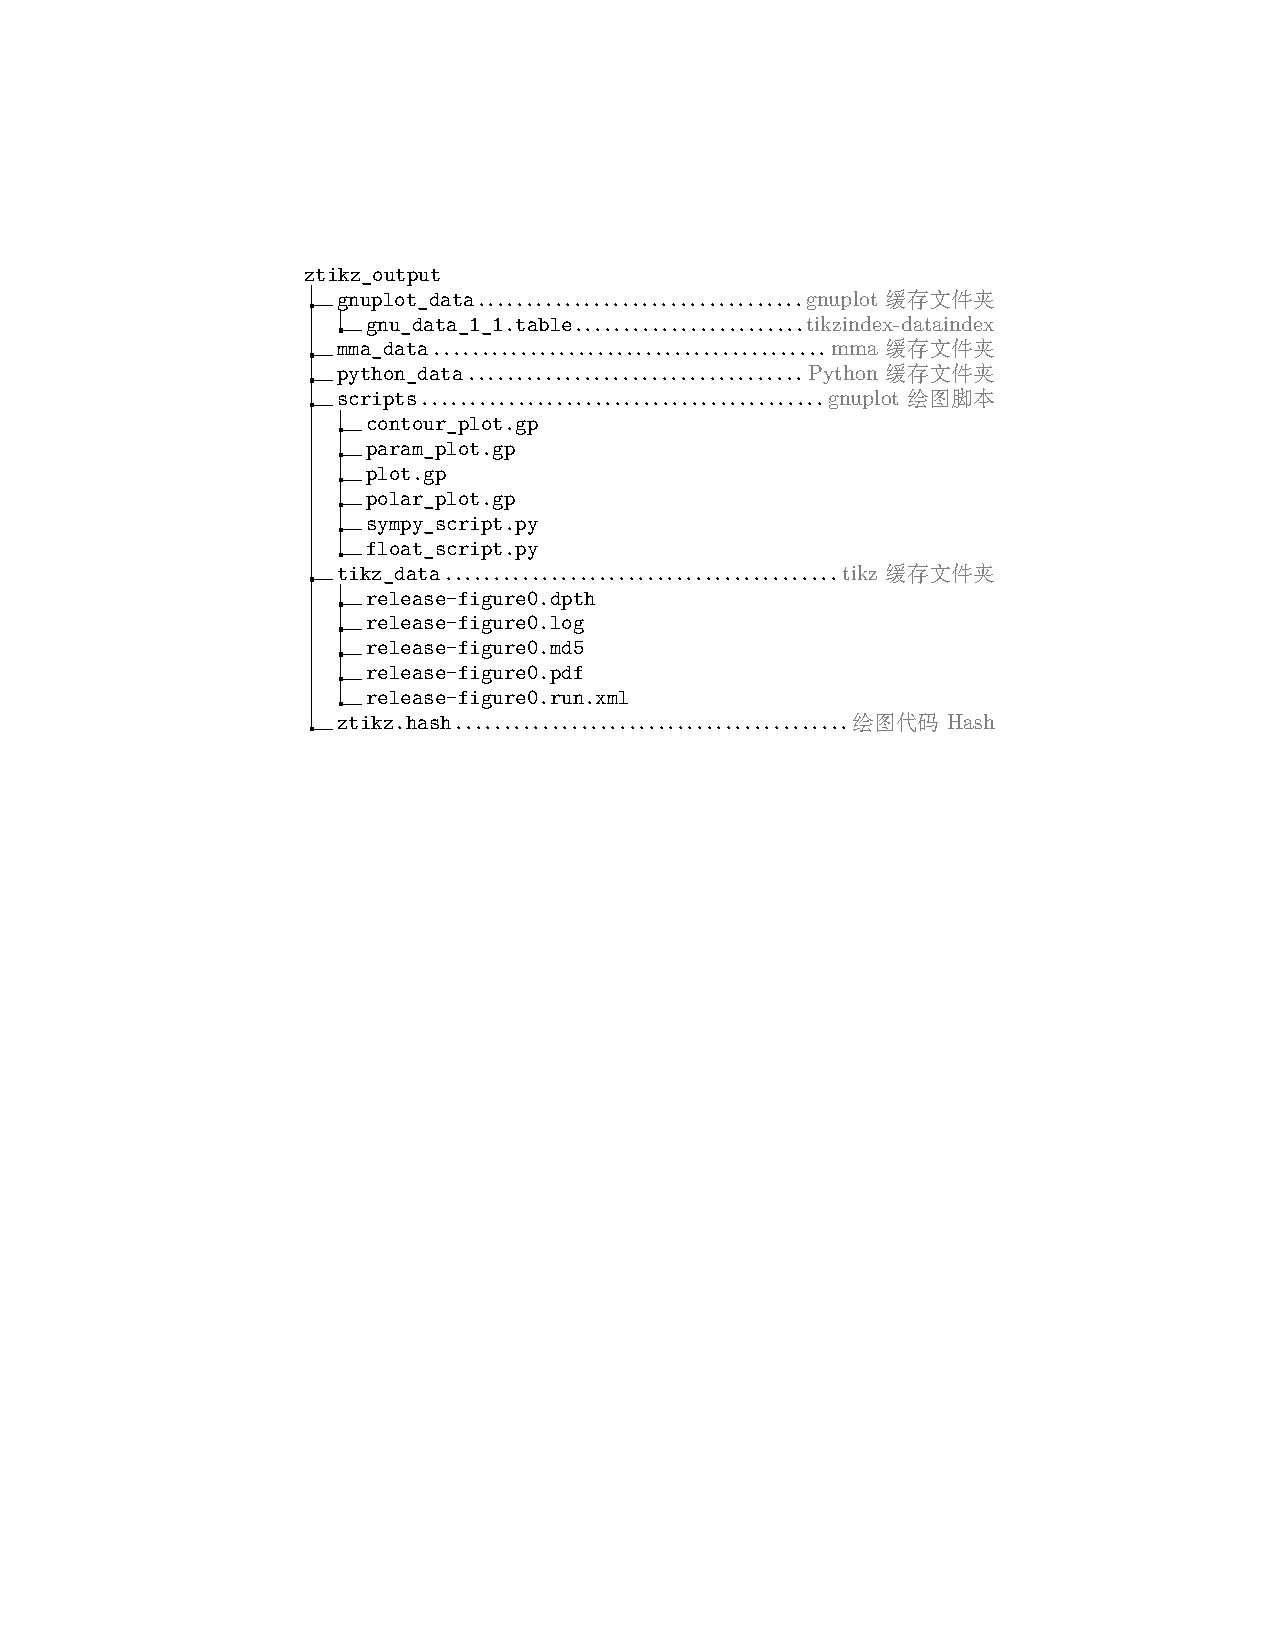
\includegraphics[width=.75\linewidth]{./ztikz_tree.pdf}
    \caption{zTikZ目录结构示意图}
    \label{fig:zTikZ-directory}
\end{figure}

{tikz\_data}中的 {release-figure0.pdf}即为缓存的 {tikzpicture}环境的pdf文件,此时在
对应的{.md5}文件中可以看到如下内容:

\begin{minted}{latex}
\def \tikzexternallastkey {AE7F2539E81C96848ADCCEE3994993D1}%
\end{minted}

此即保存的 tikzpicture 环境中代码的 Hash Value, 当我们改变 {tikzpicture}环境中的代码时,
这个Hash value就会改变,从而tikz就会再次运行此环境,重新生成图片. 这是tikz自带的功能,同时,
zTikZ中的 Cache 机制和此原理是十分类似的. 顺便说明命令:\cmd{\gnudata}的用法(在后面区域填充时是即为有用的):

\begin{minted}{latex}
\gnudata{2} = ./ztikz_output/gnuplot_data/gnu_data_1_2.table
\end{minted}

\cmd{\gnudata}参数中的``2''表示此数据是在当前tikzpicture环境中的第二个函数绘图数据; 
每一个已经绘制的函数都会在对应的文件夹下生成一个对应的数据文件,你可以使用此数据文件进行
多种操作:
\begin{itemize}
    \item 绘制此文件:\cmd{\draw plot file{\gnudata{<index>}}}.
    \item 填充此文件对应曲线:\cmd{\fill[<style>] plot file{\gnudata{<index>}}}.
    \item 绘制此文件对应散点图:只需在绘制散点图前指定绘制精度即可.
\end{itemize}

\begin{remark}
    目前由于技术原因,\cmd{\ContourPlot}命令生成的数据暂时不可用于后续填充操作.可考虑将对应隐函数转化为参数方程形式或极坐标形式,
    然后再导出对应的数据. 如果你强行使用此类型数据,那么用户可能会得到如下不良输出:
    \begin{figure}[H]
        \centering
        
\includegraphics[width=.3\linewidth]{./contour_data_bug.pdf}
        \caption{ContourPlot Fill Bug}
        \label{fig:ContourPlot Fill Bug}
    \end{figure}
\end{remark}

后续我会解释这个文件夹中其他文件的作用,目前我们先把函数绘制命令\cmd{\Plot}的参数解释清楚.
如果想要设置绘制的函数图形的样式,只需要对其第二个可选项参数进行设置即可,
比如设置为``\textcolor{red}{红色}, \textbf{加粗}''.

\begin{minted}{latex}
\begin{tikzpicture}
    \Plot[-1.5*pi:pi][red, thick]{sin(x)}
\end{tikzpicture}
\end{minted}

\begin{center}
    \begin{tikzpicture}
        \Plot[-1.5*pi:pi][red, thick]{sin(x)}
    \end{tikzpicture}
\end{center}


其实上面的第二个参数的值可以是任何合法的\cmd{\draw[<plot style>]}值, 因每一个函数
绘制命令均通过如下命令实现:

\begin{minted}{latex}
% gnuplot data rename, plot and precise reset
\cs_new_protected:Npn \ztikz_gnu_data_plot_cs:nnn #1#2#3 {
    % rename data file
    \int_gadd:Nn \g__gnu_data_index_int {1}
    \tl_set:Nx \l__gnu_data_new_name_tl {
        gnu_data_\int_use:N \g__tikz_env_index_int _
        \int_use:N \g__gnu_data_index_int.table
    }
    \tl_set:Nx \l__gnu_data_full_path_tl {\g__ztikz_gnu_path_tl/\l__gnu_data_new_name_tl}
    \sys_shell_mv:xx {\g__ztikz_gnu_path_tl/gnu_data.table}
                        {\l__gnu_data_full_path_tl}
    % plot data file
    \tl_if_empty:nTF {#3}{
        \draw[#2] plot[smooth] file {\l__gnu_data_full_path_tl};
    }{
        \group_begin:
        \keys_set:nn { ztikz / point } { #3 }
        \draw[#2] plot [
            mark = \str_use:N \l__point_type_str, 
            mark~ size = \dim_use:N \l__point_radius_dim,
            mark~ options = {
                rotate  = \fp_use:N \l__point_rotate_angle, 
                opacity = \tl_use:N \l__point_opacity_tl, 
                color   = \tl_use:N \l__point_color_tl,
                ball~ color = \tl_use:N \l__point_color_tl,
            }
        ] file {\l__gnu_data_full_path_tl};
        \group_end:
    }
    % reset precise (default 300 for plot precise)
    \bool_if:cTF {g__#1_precise_bool}{
        \PlotPrecise{#1}{100}
    }{\relax}
}
\end{minted}

上述命令 \cmd[F]{\ztikz_gnu_data_plot_cs:n} 第二个参数即为\cmd{\Plot}命令中的第二个参数;

\subsection{Show Axis}
最后给我们的图像加上坐标轴等细节: 需要用到绘制坐标轴的\cmd{\ShowAxis}命令, 绘制网格用的\cmd{\ShowGrid}命令,以及
绘制点用的\cmd{\ShowPoint}命令.

其中\cmd{\ShowAxis}\index{\cmd{\ShowAxis}}的参数格式为:\cmd{\ShowAxis[<plot style>]{(start coordinate);(end coordinate)}}.
这里的\cmd{<plot style>}参数采用键值对的形式指定,可用键值对列表以及不同键的默认值可参见如下源码声明:
\begin{minted}{latex}
% basic tick args
tickStart       .fp_set:N   = \l__start_fp,
tickStart       .initial:n  = { -5 },
tickEnd         .fp_set:N   = \l__end_fp,
tickEnd         .initial:n  = { 5 },
axisRotate      .fp_set:N   = \l__axis_rotate_angle,
axisRotate      .initial:n  = { 0 },
% tick dimension spec
mainStep        .fp_set:N   = \l__main_step_fp,
mainStep        .initial:n  = { 1.0 },
subStep         .fp_set:N   = \l__sub_step_fp,
subStep         .initial:n  = { 0.1 },
mainTickLabel   .tl_set:N   = \l__main_tick_label_tl,
mainTickLabel   .initial:n  = { \fp_use:N {\CurrentFp} },
tickLabelShift  .dim_set:N  = \l__tick_label_shift_dim,
tickLabelShift  .initial:n  = { 0pt },
mainTickLength  .dim_set:N  = \l__main_tick_length_dim,
mainTickLength  .initial:n  = { 4pt },
subTickLength   .dim_set:N  = \l__sub_tick_length_dim,
subTickLength   .initial:n  = { 2pt },
mainTickLabelPosition .tl_set:N  = \l__main_tick_label_position_tl,
mainTickLabelPosition .initial:n = { below },
% color spec
axisColor       .tl_set:N   = \l__axis_color_tl,
axisColor       .initial:n  = { black },
mainTickColor   .tl_set:N   = \l__main_tick_color_tl,
mainTickColor   .initial:n  = { black },
subTickColor    .tl_set:N   = \l__sub_tick_color_tl,
subTickColor    .initial:n  = { black },
mainTickLabelColor .tl_set:N  = \l__main_tick_label_color_tl,
mainTickLabelColor .initial:n = { black },
% tick cross type spec
tickStyle       .choice:,
tickStyle/cross .code:n     = \tl_set:Nn \l__tick_spec_tl { cross },
tickStyle/above .code:n     = \tl_set:Nn \l__tick_spec_tl { above },
tickStyle/below .code:n     = \tl_set:Nn \l__tick_spec_tl { below },
\end{minted}

一个自定义\cmd{\ShowAxis}命令示例如下:
\begin{minted}{latex}
\NewDocumentCommand{\xAxis}{O{-2}O{8}}{
    \ShowAxis[
        tickStart=\fp_eval:n {#1+1}, tickEnd=\fp_eval:n {#2-0.75}, 
        mainStep=1, subStep=.25, 
        axisRotate=0, axisColor=black,
        mainTickColor=black, subTickColor=black,
        mainTickLength=10pt, subTickLength=5pt,
        tickLabelShift=0pt, tickStyle=below, 
        mainTickLabelPosition=below
    ]{(#1, 0); (#2, 0)}
}
\end{minted}

从上述zTikZ内置的\cmd{\xAxis}\index{\cmd{\xAxis}}命令可以看出,我们可以指定坐标轴的如下属性:
\begin{itemize}
    \item 主(子)刻度绘制起点/终点
    \item 主(子)刻度颜色设置
    \item 主刻度标签颜色/位置,可选位置有:\cmd{above, below, left, right}
    \item 主(子)刻度长度
    \item 主(子)刻度间隔
    \item 主刻度坐标偏移量
    \item 主(子)刻度旋转角度,请注意调整旋转后标签的位置.
    \item 主(子)刻度样式:\cmd{cross, above, below},分别代表ticks在坐标轴的两侧还是某一侧.
\end{itemize}

\cmd{\ShowAxis}中的第二个参数表示绘制的坐标轴的起点和终点,使用``\cmd{;}''进行分割(zTikZ 中凡是单个参数中含有多个对象的,
分割对象所用到的符号都是``\cmd{;}''). zTikZ内置\cmd{\xAxis,\yAxis}\index{\cmd{\yAxis}}命令,用于绘制两条标准的坐标轴.命令的参数格式为:
\begin{minted}{latex}
\xAxis[<start>][<end>]
\yAxis[<start>][<end>]
\end{minted}

上面的\cmd{<start>, <end>}分别表示$x,y$轴对应的坐标轴绘制的起始,终止点.对应 $x$轴即为:\cmd{(<start>, 0) -- (<end>, 0)}.
$y$轴即交换坐标.

\begin{remark}
    如果在使用\cmd{\ShowAxis}命令时,没有指定可选参数中键\cmd{tickStyle}的值时,那么此时并不会绘制任何的刻度.
\end{remark}

今后用户若需要多次绘制坐标轴及其对应的标签,可以在导言区自定义一个\cmd{\ShowXYAxis}命令,
自动完成坐标轴绘制以及对应的标签.
% xyaxis
\newcommand{\ShowXYAxis}[2]{
    \ShowAxis{(-#1, 0); (#1, 0)}
    \ShowAxis{(0, -#2); (0, #2)}
    \ShowPoint[opacity=0]{(0, 0)}[$O$][below left]
    \ShowPoint[opacity=0]{(#1, 0)}[$x$][below]
    \ShowPoint[opacity=0]{(0, #2)}[$y$][left]
}

\begin{minted}{latex}
\newcommand{\ShowXYAxis}[2]{
    \ShowAxis{(-#1, 0); (#1, 0)}
    \ShowAxis{(0, -#2); (0, #2)}
    \ShowPoint[opacity=0]{(0, 0)}[$O$][below left]
    \ShowPoint[opacity=0]{(#1, 0)}[$x$][below]
    \ShowPoint[opacity=0]{(0, #2)}[$y$][left]
}
\end{minted}

然后使用命令\cmd{\ShowXYAxis}即可完成坐标轴的绘制以及对应的标注.第一个参数:$x$的绘制范围为\texttt{[-\#1, \#1]},
第二个参数:$y$的绘制范围为\texttt{[-\#2, \#2]}.默认两轴对称,如果需要更多的样式,请使用\cmd{\ShowAxis}命令进行自定义.
更多的关于坐标轴设置的样例可以参见: \cref{sec:gallery} -- Plot Gallery.

在绘制完坐标轴之后,就是网格绘制;使用\cmd{\ShowGrid}命令.\cmd{\ShowGrid}\index{\cmd{\ShowGrid}}命令的参数也是和\cmd{\ShowAxis}
命令的参数一样的,只不过此命令中可以指定一个\cmd{step}关键字,用于指定绘制网格的步长(间隔), 如\cmd{step=.5},设置步长为0.5.

\subsection{Show Point}
对应的\cmd{\ShowPoint}\index{\cmd{\ShowPoint}}命令的参数格式为:

\begin{minted}{latex}
\ShowPoint[<marker option>]{(coordinate 1); (coordinate 2); ...}[<label 1>; <label2>; ...][<position>]
\end{minted}

上述的\cmd{<marker option>>}\index{\cmd{<marker option>}}通过\cmd{<key>-<value>}的格式进行指定, 可用的\cmd{<key>-<value>}列表为:

\begin{itemize}
    \item \zkey{type}: zTikZ库已经加载\cmd{pgfmarkers}库,所以任何在此库中的形状均为有效值, 
        默认为实心 circle 样式,即\cmd{type=*}. 更多样式可以参见:\cref{fig:point-marker}(截取自pgf手册).
    \item \zkey{radius}: \cmd{dimension}, 点的半径,默认为 1pt.
    \item \zkey{color}: \cmd{color}, 点的颜色, 默认为black.
    \item \zkey{opacity}: \cmd{float value}, 点的透明度,默认为1,即不透明.
    \item \zkey{rotate}: marker的旋转角度, 默认为0.
\end{itemize}

\begin{figure}
    \centering
    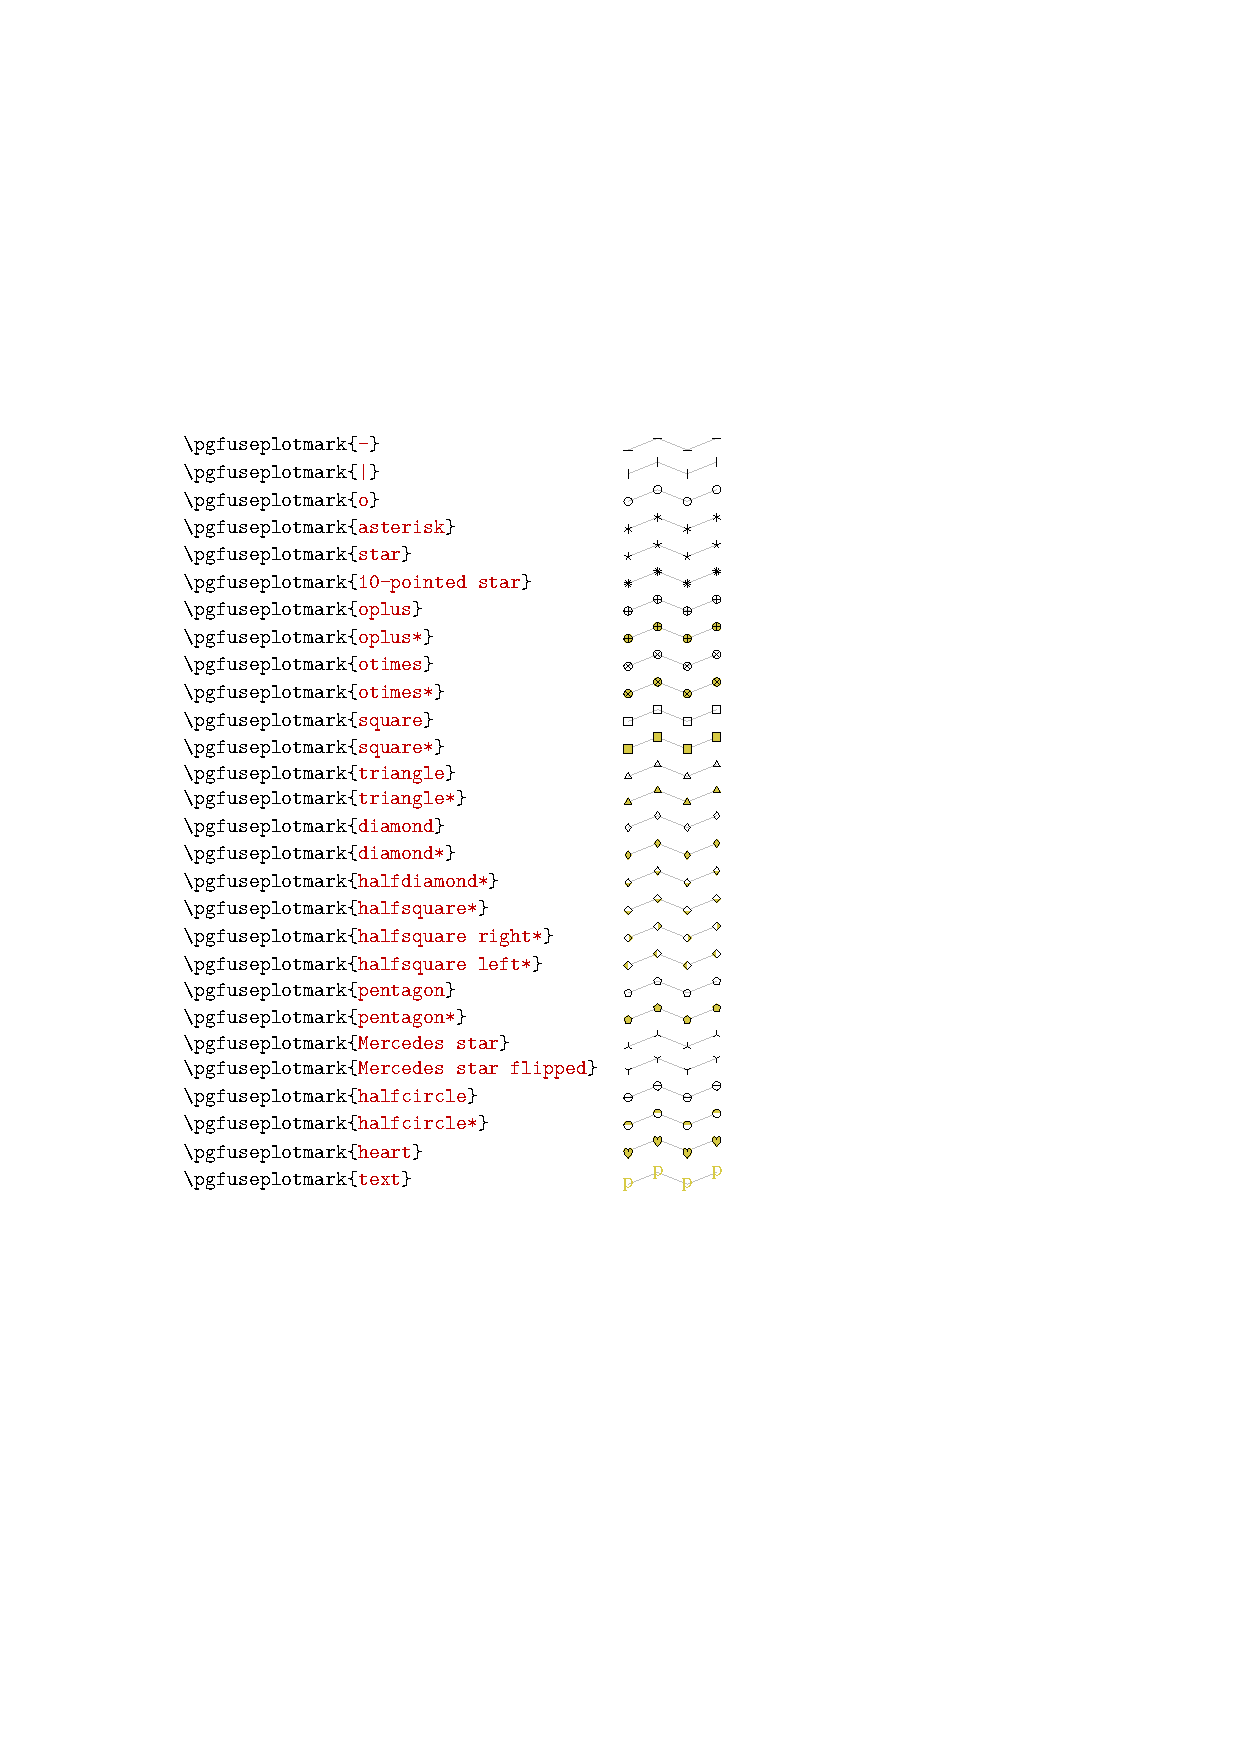
\includegraphics[width=.95\linewidth]{./point_marker.pdf}
    \caption{Point Marker}
    \label{fig:point-marker}
\end{figure}

终于,现在我们可以给出一个相对完整的代码(包括\cmd{<marker option>}对应的设置):

\begin{minted}{latex}
\begin{tikzpicture}[>=Latex]
    \xAxis[-5][5]
    \yAxis[-2][5]
    \Plot[-1.5*pi:pi][red, thick]{sin(x)}
    \ShowGrid[gray, step=1, opacity=.5]{(-5, -2); (5, 5)}
    % marker option
    \PlotPrecise{plot}{10}
    \Plot[-1.5*pi:pi][thick][type=ball, color=red]{sin(x)+.75}
    % show point
    \ShowPoint[color=teal, radius=2pt, type=pentagon*, opacity=.8, rotate=60]
        {(0, 0); (3.1415926, 0)}[$O=(0, 0)$; $(\pi, 0)$][above right=4em and 0em, font=\small]
\end{tikzpicture}
\end{minted}

\begin{center}
\begin{tikzpicture}[>=Latex]
    \xAxis[-5][5]
    \yAxis[-2][5]
    \Plot[-1.5*pi:pi][red, thick]{sin(x)}
    \ShowGrid[gray, step=1, opacity=.5]{(-5, -2); (5, 5)}
    % marker option
    \PlotPrecise{plot}{10}
    \Plot[-1.5*pi:pi][thick][type=ball, color=red]{sin(x)+.75}
    % show point
    \ShowPoint[color=teal, radius=2pt, type=pentagon*, opacity=.8, rotate=60]
        {(0, 0); (3.1415926, 0)}[$O=(0, 0)$; $(\pi, 0)$][above right=4em and 0em, font=\small]
\end{tikzpicture}
\end{center}

\begin{leftbar}
\noindent \textbf{注意:}zTikZ中的命令都不需要你使用``\cmd{;}''去结束绘制.
\end{leftbar}


\subsection{Contour Plot}
这几个函数绘制命令中,稍微值得一提的是命令:\cmd{\ContourPlot}\index{\cmd{\ContourPlot}}, 其参数格式为:

\begin{minted}{latex}
\ContourPlot[<plot domain>][<plot style>][<marker options>]{<function>}
\end{minted}

因为是 contour plot, 所以它的定义域指定格式比较特别;比如绘制的区域为:
$-3<x<\pi$ 并且 $-1.5<y<e$ 时. 那么在指定其\cmd{<plot domain>}时应写为
\cmd{-3:pi;-1.5:exp(1)}.

\begin{leftbar}
\noindent 由于zTikZ的这部分功能都是以gnuplot为基础,所以只要是gnuplot支持的函数,gnuplot内置的任何常数;
你都可以在zTikZ中使用;这里给不熟悉gnuplot的你们推荐一份7页的gnuplot快速
入门清单:\href{http://www.gnuplot.info/docs_4.0/gpcard.pdf}{gnuplot card}
\end{leftbar}

这里给出一个关于\cmd{\ContourPlot}命令的小例子:

\begin{center}
    \begin{tikzpicture}[>=Latex, scale=.5]
        \ShowAxis{(-5, 0); (5, 0)}
        \ShowAxis{(0, -5); (0, 5)}
        \ContourPlot[-3:pi; -3:exp(1)][red]{x**2/16 + y**2/10 - 1}
    \end{tikzpicture}
\end{center}

\begin{minted}{latex}
\begin{tikzpicture}[>=Latex, scale=.5]
    \ShowAxis{(-5, 0); (5, 0)}
    \ShowAxis{(0, -5); (0, 5)}
    \ContourPlot[-3:pi; -3:exp(1)][red]{x**2/16 + y**2/10 - 1}
\end{tikzpicture}
\end{minted}

对于\cmd{\ContourPlot}还有一点提醒:若要绘制方程 $x^2/4+y^2/9=1$,那么你只需输入\cmd{x**2/4+y**2/9-1},不需要对应的 = ;
所以由此也暗示了此命令的另一用法:用于绘制水平线($y=c$)和竖直线($x=c$). 仍然可以使用键\cmd{<plot domain>}
控制变量 $x,y$ 范围. 比如绘制 $x=1, -1<y<1$. 那么对应的命令为:(第一个参数$x$的范围只要包含 $x=1$即可):

\begin{minted}{latex}
\ContourPlot[0:2; -1:1][red, dashed]{x-1}
\end{minted}


\subsection{3d plot}
目前调用 gnuplot 模块进行 3d 绘制的命令\textbf{仅有}\cmd{\Plotz}, 其格式为:
\begin{minted}{latex}
\Plotz[<domain>, <palette>, <width>]{<function>}
\end{minted}

其中参数 \zkey{domain} 和命令\cmd{\ContourPlot}中的格式和意义一致. 参数\zkey{palette}用于设置绘制的调色板, 默认为 
\cmd{rgbformulae 22,13,-31}, 若想要自定义对应的调色板请参见 gnuplot 文档. 参数 \zkey{width} 接受一个合法的长度值,
如\cmd{.5\linewidth, 10cm, 100pt} 等. 

下面为两个绘制示例:
\begin{minted}{latex}
\Plotz[
  width=1\linewidth, 
  domain={-3:3; -3:3}
]{x**2+y**2-2 with pm3d, -x**2-y**2+8 with lines}

\Plotz[
  width=1\linewidth, 
  domain={-3:3; -3:3}, 
  palette={cubehelix start 0 cycles -1. saturation 1}
]{x**2-y**2-2 with pm3d}
\end{minted}

\begin{center}
\Plotz[width=.5\linewidth, domain={-3:3; -3:3}]{x**2+y**2-2 with pm3d, -x**2-y**2+8 with lines}

\Plotz[width=.5\linewidth, domain={-3:3; -3:3}, palette={cubehelix start 0 cycles -1. saturation 1}]{x**2-y**2-2 with pm3d}
\end{center}

\begin{remark}
关于绘制三维参数方程,目前不打算支持.一方面是因为目前这个模块已经比较臃肿,另一方面则是 zTikZ 没有支持三维图形绘制的计划.
\end{remark}

\subsection{Intersection}
命令没有讲到:\cmd{\ShowIntersection}\index{\cmd{\ShowIntersection}} 的使用比较简单;
其命令\cmd{\ShowIntersection}的调用格式为:

\begin{minted}{latex}
\ShowIntersection{<path 1>; <path 2>}[<number of points>]
\end{minted}

指定tikz中path名称并显示交点方法示例, 我们分别指定两条叫做\cmd{line1, line2}的路径,并显示它们二者的交点.

\begin{minted}{latex}
\begin{tikzpicture}[>=Latex]
    \ShowAxis{(-2, 0); (4, 0)}
    \ShowAxis{(0, -2); (0, 4)}
    \Plot[1:3][name path=line1]{2*x-3}
    \Plot[0:3][name path=line2]{-x+3}
    \ShowIntersection[color=red]{line1; line2}{1}

    % 可以使用如下的语句
    % \path[name intersections={of=line1 and line2}];
    % \ShowPoint[color=red] {(intersection-1)}
\end{tikzpicture}
\end{minted}


\begin{center}
  \begin{tikzpicture}[>=latex]
      \ShowAxis{(-2, 0); (4, 0)}
      \ShowAxis{(0, -2); (0, 4)}
      \Plot[1:3][name path=line1]{2*x-3}
      \Plot[0:3][name path=line2]{-x+3}
      \ShowIntersection[color=red]{line1; line2}{1}
  \end{tikzpicture}
\end{center}


\subsection{PlotPrecise}
\cmd{\PlotPrecise}\index{\cmd{\PlotPrecise}}命令主要用于指定以上一个函数绘制命令的绘制精度,其参数格式为:
\begin{minted}{latex}
\PlotPrecise{<plot type>}[<change domain>]{<samples-int>}
\end{minted}

支持的\cmd{<plot type>}:\cmd{plot, param, contour, polar}, 分别用于设置命令\cmd{\Plot, \ParamPlot, \ContourPlot, \PolarPlot}
的采样精度. 采样精度的设置分为两种,临时和永久,临时改变(只改变下一个命令的采样精度)的方法是在命令的第二个参数中
填入\cmd{[once]}; 而如果填入不是\cmd{once},那么接下来的所有同种\cmd{<plot type>}的函数绘制命令的采样精度均会受到影响. 
下面给出一个采样精度设置的例子, 绘制在区间$[-2, 2]$上的函数 $y=3\sin(1/x)$在采样精度分别为50和1000的图像,见\cref{fig:plot-precise}:

\begin{figure}[!htb]
    \centering
    \begin{tikzpicture}
        \PlotPrecise{plot}{50}
        \Plot[-2:2]{3*sin(1/x)}
    \end{tikzpicture}
    \;
    \begin{tikzpicture}
        \PlotPrecise{plot}{1000}
        \Plot[-2:2]{3*sin(1/x)}
    \end{tikzpicture}
    \caption{绘制精度设置}
    \label{fig:plot-precise}
\end{figure}


\section{Statistic Plot}
\subsection{Stairs Plot}
了解完用户曲线绘制的一系列Plot命令后,现在开始介绍和统计相关的几个绘图命令:
\cmd{\ListPlot}\index{\cmd{\ListPlot}}, \cmd{\StairsPlot}\index{\cmd{\StairsPlot}}, 
\cmd{\StemPlot}\index{\cmd{\StemPlot}}, \cmd{\BarPlot}\index{\cmd{\BarPlot}}, \cmd{\ShadePlot}\index{\cmd{\ShadePlot}}.
这几个命令在本节开篇已经介绍了其大致的功能. 本节主要聚焦于怎么使用这几个命令. 由于除\cmd{\ShadePlot,\ListPlot}外,其余3者的用法完全一致,
不同的仅仅为第一个可选参数的意义. 其中\cmd{\ListPlot}仅仅只需把对应的绘制命令中\cmd{opacity=0}即可,本节便以\cmd{\StairsPlot}为例,
讲解这三者的用法.同时也会给出3者的具体示例.

\cmd{\StairsPlot}主要用于绘制阶梯图,命令格式为:
\begin{minted}{latex}
\StairsPlot[<stairs option>][<draw option>][<marker option>]{<data>}
\end{minted}

第一个可选参数的可选值有:\cmd{plot-left(plot-right);jump-right(plot-left)},我们以``;''进行两个配置项的分割.
第一个配置项\cmd{plot-<.>}表示在绘制数据点时水平线取值为左值还是右值.第二个配置项\cmd{jump-<.>}表示在绘制数据点时
跳过左侧还是右侧的垂直线,为空时默认绘制两侧的垂直线. 

\begin{remark}
    如果两个配置项\cmd{plot-<.>, jump-<.>}均为空,那么此时绘制的图像为通过线段相连的散点图
\end{remark}

其中必选参数\cmd{<data>}表示要可视化的数据文件,可以手动输入数据文件地址,也可以使用前文定义的\cmd{\gnudata{<index>}}命令
用于引用前面已经生成的数据,\textbf{这也就意味着要使用此命令,必须先产生对应的数据}.一个绘制样例如\cref{fig:stairs-plot}:

\begin{minted}{latex}
\begin{tikzpicture}
    \ShowGrid[step=1]{(-5, -5); (5, 5)}
    %% \StairsPlot
    % 1. connected using piecewise constant series of lines
    \begin{scope}[yshift=1cm]
        \StairsPlot[plot-left;][red]{./sine.data}
        \node[left] at (-3.14, 0) {plot left(default)};
    \end{scope}
    \begin{scope}[yshift=-1cm]
        \StairsPlot[plot-right;][orange]{./sine.data}
        \node[left] at (-3.14, 0) {plot right};
    \end{scope}
    % 2. plot segment (non-connected series of lines)      
    \begin{scope}[yshift=2cm]
        \StairsPlot[;jump-left][teal][type=ball, color=teal]{./sine.data}
        \node[left] at (-3.14, 0) {jump left};
    \end{scope}
    \begin{scope}[yshift=-2cm]
        \StairsPlot[;jump-right][cyan][type=ball, color=cyan]{./sine.data}
        \node[left] at (-3.14, 0) {jump right};
    \end{scope}
\end{tikzpicture}
\end{minted}

\begin{figure}
    \centering
    \begin{tikzpicture}
        \ShowGrid[step=1]{(-5, -5); (5, 5)}
        %% \StairsPlot
        % 1. connected using piecewise constant series of lines
        \begin{scope}[yshift=1cm]
            \StairsPlot[plot-left;][red]{./sine.data}
            \node[left] at (-3.14, 0) {plot left(default)};
        \end{scope}
        \begin{scope}[yshift=-1cm]
            \StairsPlot[plot-right;][orange]{./sine.data}
            \node[left] at (-3.14, 0) {plot right};
        \end{scope}
        % 2. plot segment (non-connected series of lines)      
        \begin{scope}[yshift=2cm]
            \StairsPlot[;jump-left][teal][type=ball, color=teal]{./sine.data}
            \node[left] at (-3.14, 0) {jump left};
        \end{scope}
        \begin{scope}[yshift=-2cm]
            \StairsPlot[;jump-right][cyan][type=ball, color=cyan]{./sine.data}
            \node[left] at (-3.14, 0) {jump right};
        \end{scope}
    \end{tikzpicture}
    \caption{stairs-plot}
    \label{fig:stairs-plot}
\end{figure}

其余的两个相似命令\cmd{\StemPlot, \BarPlot}的参数格式为:
\begin{minted}{latex}
\StairsPlot[<stem/bar option>][<draw option>][<marker option>]{<data>}
\end{minted}

这里主要说明第一个可选参数的可选值列表,默认值以及其对应的实际含义.\cmd{\StemPlot}命令各参数含义如下:
\begin{itemize}
    \item \cmd{x}:表示绘制一个垂直于$x$轴上的火柴棍图
    \item \cmd{y}:表示绘制一个垂直于$y$轴上的火柴棍图
    \item \cmd{o}:表示绘制一个中心为原点 $O=(0,0)$的火柴棍图
    \item 若为空值,那么默认和\cmd{x}参数时的情形一致
\end{itemize}

其实命令 \cmd{\BarPlot} 和上述的\cmd{\Stemplot}命令的使用方法完全类似, 一般人们把这个叫做``火柴棒''图.
此命令各参数及其含义如下:
\begin{itemize}
    \item \cmd{x}:表示绘制一个垂直于$x$轴上的{\bf 离散}柱形图
    \item \cmd{y}:表示绘制一个垂直于$y$轴上的{\bf 离散}柱形图
    \item \cmd{xc}:表示绘制一个垂直于$x$轴上的{\bf 连续}柱形图
    \item \cmd{yc}:表示绘制一个垂直于$y$轴上的{\bf 连续}柱形图
    \item 若为空值,那么默认和\cmd{x}参数时的情形一致
\end{itemize}

\subsection{Stem/Bar Plot}
下面各处这两个命令的一个简单示例,见\cref{fig:bar-plot}, \cref{fig:stem-plot}:
\begin{minted}{latex}
\begin{tikzpicture}
    \ShowGrid[step=1]{(-5, -5); (5, 5)}
    %% \StemPlot
    % 1. xcomb
    \begin{scope}[yshift=-3cm]
        \StemPlot[x][red][type=*, color=red]{./sine.data}
        \node[left] at (-3.14, 0) {xcomb};
    \end{scope}
    % 2. ycomb
    \begin{scope}[yshift=0cm]
        \StemPlot[y][orange][type=*, color=orange]{./sine.data}
        \node[left] at (-3.14, 0) {ycomb};
    \end{scope}
    % 3. polar comb
    \begin{scope}[yshift=3cm]
        \StemPlot[o][cyan][type=*, color=cyan]{./sine.data}
        \node[left] at (-2, 0) {polar comb};
    \end{scope}
\end{tikzpicture}
\end{minted}

\begin{figure}[!htb]
    \centering
    \begin{tikzpicture}
        \ShowGrid[step=1]{(-5, -5); (5, 5)}
        %% \StemPlot
        % 1. xcomb
        \begin{scope}[yshift=-3cm]
            \StemPlot[x][red][type=*, color=red]{./sine.data}
            \node[left] at (-3.14, 0) {xcomb};
        \end{scope}
        % 2. ycomb
        \begin{scope}[yshift=0cm]
            \StemPlot[y][orange][type=*, color=orange]{./sine.data}
            \node[left] at (-3.14, 0) {ycomb};
        \end{scope}
        % 3. polar comb
        \begin{scope}[yshift=3cm]
            \StemPlot[o][cyan][type=*, color=cyan]{./sine.data}
            \node[left] at (-2, 0) {polar comb};
        \end{scope}
    \end{tikzpicture}
    \caption{stem-plot}
    \label{fig:stem-plot}
\end{figure}

\begin{minted}{latex}
\begin{tikzpicture}
    \ShowGrid[step=1, color=gray, opacity=.5]{(-5, -5); (5, 5)}
    % 1. xbar
    \begin{scope}[yshift=-1cm]
        \BarPlot[x][red, pattern=north west lines, pattern color=red]{./sine.data}
        \node[left] at (-3.14, 0) {xbar};
    \end{scope}
    % 2. ybar
    \begin{scope}[yshift=1cm]
        \BarPlot[y][orange, pattern=north west lines, pattern color=orange]{./sine.data}
        \node[left] at (-3.14, 0) {ybar};
    \end{scope}
    % 3. xbar interval (fill) 
    \begin{scope}[yshift=4cm]
        \BarPlot[xc][cyan, pattern=north west lines, pattern color=cyan]{./sine.data}
        \node[left] at (-3.14, 0) {xbar continuous};
    \end{scope}
    % 3. ybar interval (fill) 
    \begin{scope}[yshift=-3cm]
        \BarPlot[yc][green, pattern=north west lines, pattern color=green]{./sine.data}
        \node[left] at (-3.14, 0) {ybar continuous};
    \end{scope}
    % annotate
    \node at (2.25 ,-4.5) {Optional args:bar width, bar shift};
\end{tikzpicture}    
\end{minted}

\begin{figure}[!htb]
    \centering
    \begin{tikzpicture}
        \ShowGrid[step=1, color=gray, opacity=.5]{(-5, -5); (5, 5)}
        % 1. xbar
        \begin{scope}[yshift=-1cm]
            \BarPlot[x][red, pattern=north west lines, pattern color=red]{./sine.data}
            \node[left] at (-3.14, 0) {xbar};
        \end{scope}
        % 2. ybar
        \begin{scope}[yshift=1cm]
            \BarPlot[y][orange, pattern=north west lines, pattern color=orange]{./sine.data}
            \node[left] at (-3.14, 0) {ybar};
        \end{scope}
        % 3. xbar interval (fill) 
        \begin{scope}[yshift=4cm]
            \BarPlot[xc][cyan, pattern=north west lines, pattern color=cyan]{./sine.data}
            \node[left] at (-3.14, 0) {xbar continuous};
        \end{scope}
        % 3. ybar interval (fill) 
        \begin{scope}[yshift=-3cm]
            \BarPlot[yc][green, pattern=north west lines, pattern color=green]{./sine.data}
            \node[left] at (-3.14, 0) {ybar continuous};
        \end{scope}
        % annotate
        \node at (0, -4.5) {Optional args for the Second:bar width, bar shift};
    \end{tikzpicture}
    \caption{bar-plot}
    \label{fig:bar-plot}
\end{figure}

\subsection{List Plot}
然后讲解一下怎么绘制散点图,以\cmd{\Plot, \PolarPlot}命令为例,见\cref{fig:list-plot}:
\begin{minted}{latex}
\begin{tikzpicture}
    \ShowGrid[step=1, color=gray, opacity=.5]{(-5, -5); (5, 5)}
    \begin{scope}[yshift=-2cm]
        \PlotPrecise{plot}{10}
        \Plot[-pi:pi][opacity=0, red][type=o, color=red]{sin(x)}
    \end{scope}
    \begin{scope}[yshift=3cm]
        \PlotPrecise{polar}{15}
        \PolarPlot[0:2*pi][opacity=0, orange][type=square, color=orange]{1-sin(t)}
    \end{scope}
    % continuous condition
    \Plot[-pi:pi][red]{sin(x)}
    \PolarPlot[0:2*pi][orange]{1-sin(t)}
\end{tikzpicture}
\end{minted}

\begin{figure}[!htb]
    \centering
    \begin{tikzpicture}
        \ShowGrid[step=1, color=gray, opacity=.5]{(-5, -5); (5, 5)}
        \begin{scope}[yshift=-2cm]
            \PlotPrecise{plot}{10}
            \Plot[-pi:pi][opacity=0, red][type=o, color=red]{sin(x)}
        \end{scope}
        \begin{scope}[yshift=3cm]
            \PlotPrecise{polar}{15}
            \PolarPlot[0:2*pi][opacity=0, orange][type=square, color=orange]{1-sin(t)}
        \end{scope}
        % continuous condition
        \Plot[-pi:pi][red]{sin(x)}
        \PolarPlot[0:2*pi][orange]{1-sin(t)}
    \end{tikzpicture}
    \caption{list-plot}
    \label{fig:list-plot}
\end{figure}

\section{zdraw}
\subsection{基本命令}
zTikZ 目前包含一基于 l3draw 的子模块 zdraw, 用于满足一些比较简单的绘图需求.zdraw 模块提供了两个基本的绘制命令和一个基本环境.
\begin{itemize}
  \item \cmd{\zrule}\index{\cmd{\zrule}}: 用于绘制一个支持颜色渐变的 rule(矩形)
  \item \cmd{\zplot}\index{\cmd{\zplot}}: 绘制支持颜色渐变的形如 $y=f(x)$ 的普通函数 
\end{itemize}

zdraw 模块提供的 \cmd{\zrule} 的命令使用是比较简单的, 格式如下:
\begin{minted}{latex}
\zrule[<width>, <height>, <startColor>, <endColor>, <step>]
\end{minted}

上述参数中的 \zkey{step} 表示绘制渐变时的精度, 自然对应的数值越小,那么对应的色彩过渡越自然. 比如,用户可以使用这个命令
来定义 \cmd{\headrule}, 从而生成一个颜色渐变的fancyhead rule. 具体代码如下:

\begin{minted}{latex}
\pagestyle{fancy}
\setlength{\headheight}{25pt}
\def\headrule{\zdrawSetUnit{pt}\zrule[width=\textwidth, step=1, height=1]}
\end{minted}

下面例举一个\cmd{\zrule}命令的使用示例,以此来说明此命令中各个参数的含义:
\begin{minted}{latex}
\zrule[width=10, startColor=red, step=1]
\end{minted}

\begin{center}
\zrule[width=10, startColor=red, step=1]
\end{center}

关于命令 \cmd{\zplot} 的使用细节请参见:\cref{subsec:l3-zplot}. 这里介绍如何设置 \cmd{\zplot} 绘图时的单位以及绘制的线径参数.
zdraw 提供 \cmd{\zdrawSetUnit, \zdrawSetPathWidth} 用于设置坐标单位和线径. 一个基本的使用样例见下:

\begin{minted}{latex}
\zdrawSetUnit{cm}
\zdrawSetPathWidth {5pt}
\end{minted}

l3draw 中默认的线径为 \cmd{0.4pt}. 那么怎么设置 l3draw 中默认的单位坐标尺寸呢? 参见如下代码:
\begin{minted}{latex}
\draw_xvec:n {2cm, 0}
\draw_yvec:n {0, 2cm}
... 
\draw_path_lineto:n {\draw_point_vec:nn {<x-coor>}{<y-coor>}}
...
\end{minted}

上述的 \cmd{x-coor, y-coor}即代表纯数字的坐标值. 通过修改上述代码中$x$-axis方向的基向量\cmd[F]{\draw_xvec:n {2cm, 0}}或 $y$-axis 方向的
基向量,用户即可以自定义绘图的单位坐标尺寸.

\subsection{基本环境}
zdraw 同时也提供了一个基本的 \cmd{zdraw}\index{\cmd{\zplot}} 环境,用于用户自由书写对应的绘图代码. 在提供本环境的同时
zdraw 模块对原 l3draw 宏包中的部分命令以及部分 \LaTeX{}3 中的命令进行了封装. 源码声明如下:
\begin{minted}{latex} 
%% draw env 
\NewDocumentEnvironment{zdraw}{O{}}{\ExplSyntaxOn\draw_begin:}{\draw_end:\ExplSyntaxOff}
\NewDocumentEnvironment{zscope}{O{}}{\draw_path_scope_begin:}{\draw_path_scope_end:}

%% cmd alias
% point/line
\cs_new_eq:NN \moveto \draw_path_moveto:n
\cs_new_eq:NN \lineto \draw_path_lineto:n
\cs_new_eq:NN \scolor \color_stroke:n
\cs_new_eq:NN \fcolor \color_fill:n

% base vector
\cs_new_eq:NN \xvec   \draw_xvec:n
\cs_new_eq:NN \yvec   \draw_yvec:n
% both follows ref (0, 0)
\cs_new_eq:NN \polar  \draw_point_polar:nn 
\cs_new_eq:NN \coor   \draw_point_vec:nn  

% shape and text
\cs_new_eq:NN \rec \draw_path_rectangle_corners:nn
\cs_new_eq:NN \cir \draw_path_circle:nn
\cs_new_eq:NN \newtext    \coffin_new:N
\cs_new_eq:NN \sethtext   \hcoffin_set:Nn
\cs_new_eq:NN \setvtext   \vcoffin_set:Nnn
\cs_new_eq:NN \scaletext  \coffin_scale:Nnn
\cs_new_eq:NN \puttext    \draw_coffin_use:Nnnn

% path operation
% scope
\cs_new_eq:NN \bg \draw_path_scope_begin:
\cs_new_eq:NN \eg \draw_path_scope_end:
% segement connect
\cs_new_eq:NN \capbutt   \draw_cap_butt:
\cs_new_eq:NN \caproun   \draw_cap_round:
\cs_new_eq:NN \caprect   \draw_cap_rectangle:
\cs_new_eq:NN \closepath \draw_path_close:
% transformatio
\cs_new_eq:NN \shift     \draw_transform_shift:n
\cs_new_eq:NN \xscale    \draw_transform_xscale:n
\cs_new_eq:NN \yscale    \draw_transform_yscale:n
\cs_new_eq:NN \trans     \draw_transform_matrix:nnnn
\NewDocumentCommand{\usepath}{O{draw}}{
  \draw_path_use_clear:n {#1}
}
\end{minted}

上述的命令:\cmd{\trans{a}{b}{c}{d}}需要稍微说明, 此命令表示对整个坐标系统进行一个线性变换, 其所对应
的变换矩阵$T$ 如下:

\[
  T = \begin{bmatrix}
    a & c \\
    b & d
  \end{bmatrix}
\]

其余的命令请参见具体文档, 这里以一个基本的例子--绘制 Venn 图,来讲解上述命令的基本使用方法. 
\begin{minted}{latex}
% union 
\begin{zdraw}
  \xscale {0.5}
  \yscale {0.5}
  \cir {2cm, 0}{2cm}
  \cir {3.5cm, 0}{2cm}
  \usepath[draw, clip]
  \fcolor {teal!50}
  \rec {-10cm, -10cm}{10cm, 10cm}
  \usepath[fill]
\end{zdraw}

% intersection 
\begin{zdraw}
  \xscale {0.5}
  \yscale {0.5}
  \cir {3.5cm, 0}{2cm}
  \usepath[draw]
  \cir {2cm, 0}{2cm}
  \usepath[clip, draw]
  \fcolor {orange}
  \cir {3.5cm, 0}{2cm}
  \usepath[fill]
\end{zdraw}

% difference
\begin{zdraw}
  \xscale {0.5}
  \yscale {0.5}
  \draw_evenodd_rule:
  \fcolor {pink}
  \cir {2cm, 0}{2cm}
  \cir {3.5cm, 0}{2cm}
  \usepath[draw, fill]
\end{zdraw}
\end{minted}

绘制效果如下:
\begin{center}
% union 
\begin{zdraw}
  \xscale {0.5}
  \yscale {0.5}
  \cir {2cm, 0}{2cm}
  \cir {3.5cm, 0}{2cm}
  \usepath[draw, clip]
  \fcolor {teal!50}
  \rec {-10cm, -10cm}{10cm, 10cm}
  \usepath[fill]
\end{zdraw}
% intersection 
\begin{zdraw}
  \xscale {0.5}
  \yscale {0.5}
  \cir {3.5cm, 0}{2cm}
  \usepath[draw]
  \cir {2cm, 0}{2cm}
  \usepath[clip, draw]
  \fcolor {orange}
  \cir {3.5cm, 0}{2cm}
  \usepath[fill]
\end{zdraw}
% difference
\begin{zdraw}
  \xscale {0.5}
  \yscale {0.5}
  \draw_evenodd_rule:
  \fcolor {pink}
  \cir {2cm, 0}{2cm}
  \cir {3.5cm, 0}{2cm}
  \usepath[draw, fill]
\end{zdraw} 
\end{center}

目前,在 l3draw 中插入文本是通过插入一个 coffins 或者是 box 实现的,下面显示一个插入文本的建档示例:
\begin{minted}{latex}
\begin{zdraw}
  \xscale {.5}
  \yscale {.5}
  \cir {-2cm, 0}{2.5cm}
  \cir {2cm, 0}{2.5cm}
  \cir {0, -2*sqrt(3)cm}{2.5cm}
  % text
  \newtext \texta
  % \sethtext \texta {$y=\alpha x + \beta$\\ Hello~ world}
  \setvtext \texta {6em}{$y=\alpha x + \beta$\\ Hello~ world}
  \scaletext \texta {2}{2}
  \puttext \texta {hc}{b}{0, -7cm}
  \usepath[draw]
\end{zdraw}
\end{minted}

具体效果如下:
\begin{center}
  \begin{zdraw}
    \xscale {.5}
    \yscale {.5}
    \cir {-2cm, 0}{2.5cm}
    \cir {2cm, 0}{2.5cm}
    \cir {0, -2*sqrt(3)cm}{2.5cm}
    % text
    \newtext \texta
    % \sethtext \texta {$y=\alpha x + \beta$\\ Hello~ world}
    \setvtext \texta {6em}{$y=\alpha x + \beta$\\ Hello~ world}
    \scaletext \texta {2}{2}
    \puttext \texta {hc}{b}{0, -7cm}
    \usepath[draw]
  \end{zdraw}
\end{center}

\begin{remark}
目前这些命令的设置是不太合理的,也仅为了我个人使用方便. 所以如果用户想要深入了解 l3draw,那么还请自行阅读其对应的文档,
而非使用 zdraw 模块中``封装''(alias)的如上命令.
\end{remark}

\subsection{pgf Shade Plot (deprecated)}
zTikZ 之前的 gnuplot 模块默认提供了一个基于 pgf 的\cmd{\ShadePlot}命令,参数格式为:
\begin{minted}{latex}
\ShadePlot[<shade mode>][<box distance>]{<data>}
\end{minted}

其中第一个参数\cmd{<shade mode>}使用命令\cmd{\ztikzShadeMode}命令进行声明,此命令的一个样例为(zTikZ默认shade模式):
\begin{minted}{latex}
\ztikzShadeMode{defaultMode}{horizontal}{white,black}
\end{minted}

\cmd{\ztikzShadeMode}的第二个参数可以为\cmd{vertical},表示垂直渐变.第三个参数中的颜色也可以超过两个.一个具体的
使用样例,见\cref{fig:shade-plot}:

\begin{minted}{latex}
% compile with "\usepackage[external=false]{ztikz}"
\ztikzShadeMode{newyMode}{vertical}{white,black}
\begin{tikzpicture}
    \ShowGrid[step=1, color=gray, opacity=.5]{(-5, -5); (5, 5)}
    \ShadePlot[newyMode][10pt]{./sine.data}
\end{tikzpicture} 
\end{minted}

\begin{figure}[!htb]
    \centering
    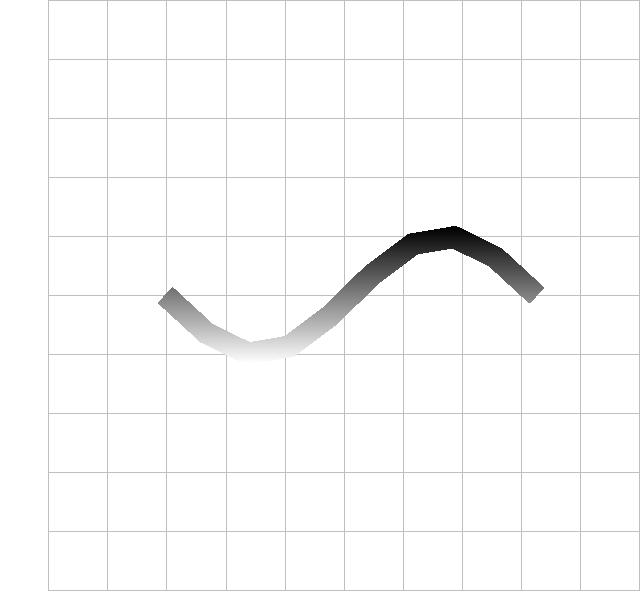
\includegraphics[width=.75\linewidth]{./ztikz_example_5.pdf}
    \caption{shade-plot}
    \label{fig:shade-plot}
\end{figure}

目前此命令可能会存在部分的潜在问题,请谨慎使用此命令(比如此命令不支持\cmd{external}库的缓存功能). 
如果想要创建一个shade区域,直接使用 \cmd{\shade}命令来代替\cmd{\fill}命令即可.在指定\cmd{\shade[<shade mode>] ...}命令
中的\cmd{<shade mode>}时可以为:\cmd{top color=red, bottom color=blue}或者是\cmd{left color=red, right color=blue}.

\begin{remark}
目前基于 pgf 的 \cmd{\shadeplot} 命令已经被废弃,因为其在绘制时会出现一些兼容性问题,但是在后续的 implement 节我仍然把之前的实现细节给出了.
如果使用者有类似的需求,那么请使用模块 zdraw 中此命令的新的实现方法\cmd{\zplot}, 而非此命令原始实现. 但是其实 zdraw 模块中的 shade 模式也并
不是正真意义上的 gradient shading, 而是通过多段 gradient segements拼接而成的.什么时候 zdraw 能支持真正意义上的 gradient? 这取决于 l3draw 
官方是否考虑加入此功能,毕竟这个功能需要一些  PDF management 的东西.详情请参见: \href{https://tex.stackexchange.com/q/719488/294585}{smooth gradient in l3draw}. 
\end{remark}

\subsection{l3daw Shade Plot}\label{subsec:l3-zplot}
由于上述基于 pgf 的\cmd{\shadeplot}命令的种种局限性. 目前 zdraw 模块已通过l3draw模块实现了曲线的渐变填充(并不是在原理层面
解决的,l3draw(\LaTeX{}3))官方正在考虑是否加入此功能).但是由于l3draw模块的限制,目前在l3draw模块中实现的命令还不支持
在tikz环境中使用. zdraw 模块中提供的命令 \cmd{\zplot} 的格式为:
\begin{minted}{latex}
\zplot[<domain>, <range>, <action>, <startColor>, <endColor>, <axis>]{<function>}
\end{minted}

上述的其余参数均与命令 \cmd{\zrule} 中参数的意义一致, 需要介绍的重点参数为 \zkey{range}. 此参数表示所绘制函数的范围.
这个参数在指定颜色的渐变范围时是比较有用的.

\begin{remark}
但是总的说来:这个颜色渐变这个功能你其实并不是经常使用的
\end{remark}

在l3draw中实现的命令\cmd[F]{\function_plot:nnn} 可以完成水平方向和垂直方向的渐变,一个具体的示例如下
\begin{minted}{latex}
\zplot[domain={0, 0.02*\c_pi_fp, 2*\c_pi_fp}, action=shade, startColor=blue, endColor=green, axis=x]{sin(x)}
\zplot[domain={0, 0.02*\c_pi_fp, 2*\c_pi_fp}, action=shade, startColor=blue, endColor=green, axis=y]{sin(x)}
\end{minted}

具体绘制效果见\cref{fig:l3-gradient}:
\begin{figure}[!htb]
  \centering
  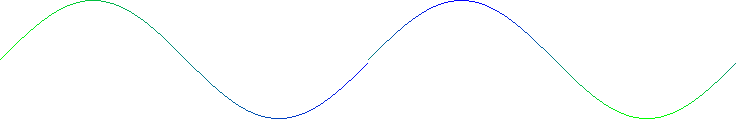
\includegraphics[width=.75\linewidth]{./l3-gradient-example.pdf}
  \caption{l3draw gradient}
  \label{fig:l3-gradient}
\end{figure}

关于此命令的具体实现,请参见\cref{code:l3-draw-implement}. 当然,你也可以指定 \cmd{startColor,endColor}为同一个颜色,
从而绘制普通的函数曲线. 如果要实现更多的渐变方式,比如沿着曲线渐变,可以参考如下示例:
\begin{minted}{latex}
% \usepackage{l3draw}
\ExplSyntaxOn
\seq_set_split:Nnn \l_tmpa_seq {;}{
  0.00000, 0.00000;
  0.03015, 0.00990;
  -0.04733, -2.98255;
  ...
  0.89511, -2.87871;
  1.76708, -2.48152;
  2.47872, -1.82505;
  2.95459, -0.97038;
  3.14159, -0.00000
}
% color gradient
\cs_set:Npn \color_gradient:n #1 {
  \color_select:n {blue!#1!green}
}
\cs_generate_variant:Nn \seq_set_split:Nnn {Nnx}
\cs_generate_variant:Nn \draw_path_moveto:n {x}
\cs_generate_variant:Nn \color_gradient:n {x}

\draw_begin:
\draw_cap_round:
% base
\draw_xvec:n {2cm, 0}
\draw_yvec:n {0, 2cm}
% draw
\draw_path_moveto:n {\draw_point_vec:nn {0.785}{0}}
\int_step_inline:nnn {2}{\fp_eval:n {\seq_count:N \l_tmpa_seq-1}}{
  \seq_set_split:Nnx \l_tmpb_seq {,}{\seq_item:Nn \l_tmpa_seq {#1}} 
  \seq_set_split:Nnx \l_tmpc_seq {,}{\seq_item:Nn \l_tmpa_seq {\fp_eval:n {#1+1}}} 
  \color_gradient:x {\fp_eval:n {#1*100/\seq_count:N \l_tmpa_seq}}
  \draw_path_moveto:n {
    \draw_point_vec:nn {\seq_item:Nn \l_tmpb_seq {1}}{\seq_item:Nn \l_tmpb_seq {2}}
  }
  \draw_path_lineto:n {
    \draw_point_vec:nn {\seq_item:Nn \l_tmpc_seq {1}}{\seq_item:Nn \l_tmpc_seq {2}}
  }
  \draw_path_use_clear:n {draw} 
}
\draw_path_use_clear:n {draw}
\draw_end:
\ExplSyntaxOff
\end{minted}

具体效果为:
\begin{figure}[!htb]
  \centering
  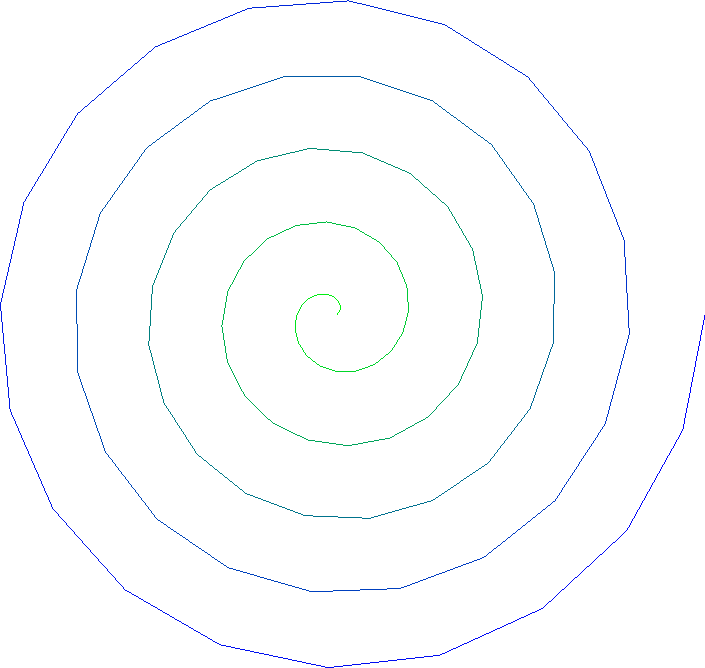
\includegraphics[width=.6\linewidth]{./curve_gradient.pdf}
  \caption{Curve Gradient}
  \label{fig:curve-gradient}
\end{figure}

\section{Polygon}
\subsection{基本介绍}
目前zTikZ的\cmd{Polygon}命令已经开发完毕, 此命令主要用于绘制正多边形.命令格式如下:
\begin{minted}{latex}
\Polygon[<options>]{<edges>}
\end{minted}

第二个参数是比较简单的,只需要输入一个正整数即可,表示多边形的边数. 第一个参数是一个可选参数,可以指定旋转角度,多边形的边长,边的颜色
多边形填充样式与颜色,顶点样式等.可用的键值对以及默认值如下:

\begin{minted}{latex}
\keys_define:nn { ztikz / polygon }{
    radius       .fp_set:N  = \l__polygon_radius_fp,
    radius       .initial:n = { 1 },
    edgeColor    .tl_set:N  = \l__polygon_edge_color_tl,
    edgeColor    .initial:n = { black },
    fillColor    .tl_set:N  = \l__polygon_fill_color_tl,
    fillColor    .initial:n = {  },
    fillOpacity  .fp_set:N  = \l__polygon_fill_opacity_fp,
    fillOpacity  .initial:n = { 0 },
    rotate       .fp_set:N  = \l__polygon_rotate_angle,
    rotate       .initial:n = { 0 },
    shift        .tl_set:N  = \l__polygon_shift_tl,
    shift        .initial:n = { (0,0) },
    marker       .tl_set:N  = \l__polygon_marker_option_tl,
    marker       .initial:n = { },
}
\end{minted}

这里指的说一下的参数是:\zkey{marker},此参数中可以填入任意合法的\cmd{<marker option>}键值对,一下为一个简单示例:
\begin{minted}{latex}
\Polygon [
    radius=2, 
    shift={(3,0)}, 
    rotate=60, 
    marker={type=ball, color=red}, 
    edgeColor=teal, 
    fillColor=red, 
]{3}
\end{minted}

\begin{remark}
  多边形的变数必须为整数. 同时再说明一下键\zkey{shift}的含义:合法的值为一个使用``()''包括的向量,表示 
  整个多边形的平移量.比如\cmd{shift={(3,-4)}}表示整个多边形向右平移3个单位,象下平移4个单位. 不要忘记向量
  外层的大括号:\texttt{\{\}}. 
\end{remark}

\begin{remark}
  其实也可以考虑把这个多边形的边数拓展为分数,甚至是负数.
\end{remark}

\subsection{使用样例}
在讲述了\cmd{\Polygon}命令的用法后,下面给出一个简单的使用样例,见\cref{fig:polygon}:
\begin{minted}{latex}
\begin{tikzpicture}
    \ShowGrid[step=1, color=gray, opacity=.5]{(-5, -5); (5, 5)}
    \Polygon[shift={(0, 0)}]{3}
    \Polygon[shift={(3, 0)}, fillColor=red, fillOpacity=.5]{4}
    \Polygon[shift={(0, 3)}, edgeColor=green, fillOpacity=.3, marker={type=ball, color=green}, rotate=18]{5}
    \Polygon[shift={(-3,0)}, fillColor=orange]{6}
    \Polygon[shift={(0,-3)}, fillColor=teal, marker={type=oplus*, color=teal}]{8}
\end{tikzpicture}
\end{minted}

\begin{figure}[!htb]
    \centering
    \begin{tikzpicture}
        \ShowGrid[step=1, color=gray, opacity=.5]{(-5, -5); (5, 5)}
        \Polygon[shift={(0, 0)}]{3}
        \Polygon[shift={(3, 0)}, fillColor=red, fillOpacity=.5]{4}
        \Polygon[shift={(0, 3)}, edgeColor=green, fillOpacity=.3, marker={type=ball, color=green}, rotate=18]{5}
        \Polygon[shift={(-3,0)}, fillColor=orange]{6}
        \Polygon[shift={(0,-3)}, fillColor=teal, marker={type=oplus*, color=teal}]{8}
    \end{tikzpicture}
    \caption{polygon}
    \label{fig:polygon}
\end{figure}


\begin{remark}
填充多边形时,若没有指定\cmd{fillColor}时,则不填充色彩.当指定\cmd{fillColor}时,
默认填充透明度为 0.75. 用户可以重新指定其透明度值,Override It. 比如,你想要填充一个透明度为50\%的多边形,那么可以
使用\cmd{fillOpacity=0.5}来实现.
\end{remark}

\section{pyfig}
\subsection{基本介绍}
python绘图是比较就简单的,zTikZ提供了用于python绘图的\cmd{pyfig}\index{\cmd{pyfig}}环境.
此环境需要填入两个参数,参数格式为:

\begin{minted}{latex}
\begin{pyfig}[<width>]{<export file name>}
% your code
\end{pyfig}
\end{minted}

其中的\cmd{<width>}参数是命令\cmd[F]{\includegraphics[<width>]{}}中的 width 参数,比如你可以输入\cmd{width=.75\linewidth}. 
在指定必要的参数后,便可以直接在环境中输入Python代码. 下面即为一个示例:

\begin{minted}{latex}
\begin{pyfig}[width=.45\linewidth]{pycode.py}
import matplotlib 
matplotlib.use('Agg')
from matplotlib import pyplot as plt
plt.rcParams['font.sans-serif'] = ['FangSong']  
plt.rcParams['axes.unicode_minus'] = False
import numpy as np

x = np.linspace(0, 2*np.pi, num = 80)
y = np.sin(x)*np.cos(x)+.2
plt.plot(x, y)
\end{pyfig}
\end{minted}

你不需要在源代码中输入图片的保存指令:\cmd{plt.savefig("")}, zTikZ会自动在此环境后面加上对应的
图片保存指令.这个环境的返回结果为:\cmd[F]{\includegraphics[width=.45\linewidth]{pycode.py.pdf}},
所以你可以把这个环境嵌套在任何的浮动环境,比如\cmd{figure, table}中. 

\subsection{缓存机制}
下面说一说这个 pyfig 环境的缓存机制. 在命令行中第一次编译此示例时你会看到如下的日志输出:
\begin{minted}{latex}
current hash is FF7B5ECDBF52AA95DF921FCC076F9021
current hash is unique --> recorded
\end{minted}

上述日志说明,zTikZ已经识别到这是一个新的python环境,并且保存了这个环境中绘图代码的Hash值;
然后,第二次编译此文档时,你会在输出的日志中定位到如下的输出:
\begin{minted}{latex}
current hash is FF7B5ECDBF52AA95DF921FCC076F9021
skip recompile by python, using the cache picture 1
\end{minted}

这就说明,由于你的python绘图部分的源代码没有改变,然后zTikZ就直接采用了上一次编译的缓存图片,跳过了重新编译这一步;
上面环境的运行结果参见:\cref{fig:py-fig-1}

\begin{figure}[!htb]
    \centering
\begin{pyfig}[width=.6\linewidth]{pycode.py}
import matplotlib 
matplotlib.use('Agg')
from matplotlib import pyplot as plt
plt.rcParams['font.sans-serif'] = ['FangSong']  
plt.rcParams['axes.unicode_minus'] = False
import numpy as np

x = np.linspace(0, 2*np.pi, num = 80)
y = np.sin(x)*np.cos(x)+.2
plt.plot(x, y)
\end{pyfig}
    \caption{Python绘图示例 1}
    \label{fig:py-fig-1}
\end{figure}

\subsection{3D 绘图示例}
这里再给一个Python绘图示例, 绘制了一个来自Matplotlib官方的简单三维图像. 
这里给出这个例子,就是为了让用户明白,尽管 zTikZ 没有提供便捷的用户绘制三维矢量图的接口,
但是你可以使用 Python 生成对应的3维矢量图;虽然,你可能需要再去学习Python中Matplotlib的
相关语法,但是这是简单的.

\begin{figure}[!htb]
    \centering
    \input{./pyfig_II.mpl}
    \caption{Python绘图示例 2}
    \label{fig:py-fig-2}
\end{figure}


\subsection{注意事项}
由于python是依靠缩进来识别代码结构的,所以在书写这部分的代码时,不能够人工添加缩进,在书写的时候
需写为\cref{fig:python-index}这样.

\begin{figure}[!htb]
  \centering
  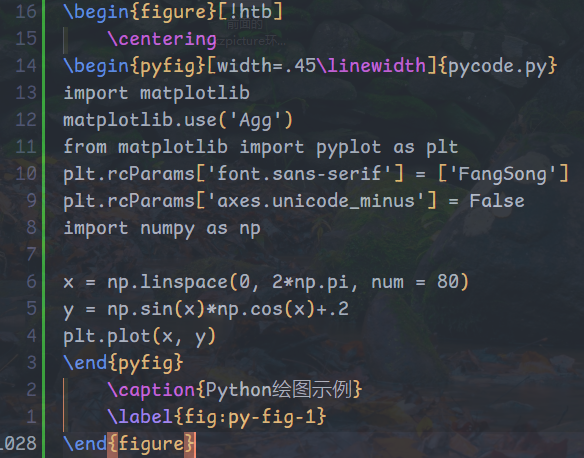
\includegraphics[width=.4\linewidth]{./pyfig_example.png}
  \caption{Python Indent}
  \label{fig:python-index}
\end{figure}

如果你实在是需要缩进,那么在这里我推荐另外一种可以使用缩进的方法:把\cmd{pyfig}环境连同其内部代码保存在另外一个文件中,
比如这里我保存为\cmd{pycode.mpl},然后在\cmd{figure}环境中使用\cmd[F]{\input{pycode.mpl}}引入此部分的代码,示例如下:
\begin{minted}{latex}
\begin{figure}
  \input{./pycode.mpl}
\end{figure}
\end{minted}


\section{wolframGraphics}
\subsection{基本介绍}
其实使用mathematica进行绘图这个部分和前面的使用Python绘图是差不多的,zTikZ提供了一个\cmd{wolframGraphics}\index{\cmd{wolframGraphics}}
环境用于调用 mathematica 进行绘图. 与之前\cmd{pyfig}环境不同的是:此时你需加入保存图片的命令,路径前缀为:\cmd{./ztikz_output/mma_data/<figure name>}. 
为何这里我不使用zTikZ自动完成? 由于mathematica绘图代码中可能存在着多幅图形需要互相组合的情况,可能会使用\cmd{Show}命令组合成为最终的目标图形, 
但是这个组合方式就多种多样了.

所以为给用户提供更多自由空间,这里的图片保存命令由用户自己书写. 并且上述\cmd{<figure name>}只能写为\cmd{<wls script name>.pdf} 的形式;
比如你的 WolframScript 脚本名称为\cmd{mma_1.wls},那么你的\cmd{<figure name>}只能写为\cmd{mma_1.wls.pdf},其中的图片格式可以自己指定,
可以为:\cmd{.png, .jpg, .mbp}等. 此环境同样支持 cache 模块.


\subsection{环境测试}
用户如果要使用zTikZ的Mathematica模块,请务必确保wolframscript在命令行中能够正常运行.可以使用如下
文件作为测试用例,检测wolframscript是否正常工作; 
\begin{minted}{mathematica}
plotFunction[fun_, xlimits_, ylimits_] := ContourPlot[fun, 
    xlimits, ylimits,
    ContourStyle->{
        RGBColor["#00C0A3"], 
        Thickness[0.004]
    },
    AspectRatio->((xlimits[[2]]//Abs) + (xlimits[[3]]//Abs))/((ylimits[[2]]//Abs) + (ylimits[[3]]//Abs)), 
    AxesOrigin->{0,0}, 
    Axes->True,
    Frame->False,
    AxesStyle->Arrowheads[{0, 0.03}],
    AxesLabel->{"x", "y"},
    PlotRange -> Full
]

xlimits = {x, -3, 6};
ylimits = {y, -4, 5};
fp1 = plotFunction[y==Sin[x], xlimits, ylimits];
fp2 = plotFunction[x^2/4 + y^2/3 == 5, {x, -5, 5}, {y, -5, 5}];

figure = Show[fp2, fp1];
(* 1.保存的图片格式为:*.wls.pdf; 2.保存路径在:./ztikz_output/mma_data *)
Export["works_well.pdf", figure];
\end{minted}

把这里的源码保存为\cmd{test.wls},然后在命令行运行:
\begin{minted}{shell}
wolframscript -script test.wls
\end{minted}

如果正常工作的话,那么在你的当前工作目录下会产生一个名为\cmd{works_well.pdf}的pdf文件.反之,你的wolframscript没有
正常配置或者是激活,也就不能够使用本模块.


\subsection{2D 绘图示例}
在介绍了 wolfram 模块的绘图功能后,下面给出一个具体的使用案例:

\begin{minted}{latex}
\begin{wolframGraphics}[width=.4\linewidth]{mma_1.wls}
    plotFunction[fun_, xlimits_, ylimits_] := ContourPlot[fun, 
        xlimits, ylimits,
        ContourStyle->{
            RGBColor["#00C0A3"], 
            Thickness[0.004]
        },
        AspectRatio->((xlimits[[2]]//Abs) + (xlimits[[3]]//Abs))/((ylimits[[2]]//Abs) + (ylimits[[3]]//Abs)), 
        AxesOrigin->{0,0}, 
        Axes->True,
        Frame->False,
        AxesStyle->Arrowheads[{0, 0.03}],
        AxesLabel->{"x", "y"},
        PlotRange -> Full
    ]
    
    xlimits = {x, -3, 6};
    ylimits = {y, -4, 5};
    fp1 = plotFunction[y==Sin[x], xlimits, ylimits];
    fp2 = plotFunction[x^2/4 + y^2/3 == 5, {x, -5, 5}, {y, -5, 5}];
    
    figure = Show[fp2, fp1];
    (* 1.保存的图片格式为:*.wls.pdf; 2.保存路径在:./ztikz_output/mma_data *)
    Export["./ztikz_output/mma_data/mma_1.wls.pdf", figure];
\end{wolframGraphics}
\end{minted}

\begin{figure}[!htb]
    \centering
    \begin{wolframGraphics}[width=.5\linewidth]{mma_1.wls}
        plotFunction[fun_, xlimits_, ylimits_] := ContourPlot[fun, 
            xlimits, ylimits,
            ContourStyle->{
                RGBColor["#00C0A3"], 
                Thickness[0.004]
            },
            AspectRatio->((xlimits[[2]]//Abs) + (xlimits[[3]]//Abs))/((ylimits[[2]]//Abs) + (ylimits[[3]]//Abs)), 
            AxesOrigin->{0,0}, 
            Axes->True,
            Frame->False,
            AxesStyle->Arrowheads[{0, 0.03}],
            AxesLabel->{"x", "y"},
            PlotRange -> Full
        ]
        
        xlimits = {x, -3, 6};
        ylimits = {y, -4, 5};
        fp1 = plotFunction[y==Sin[x], xlimits, ylimits];
        fp2 = plotFunction[x^2/4 + y^2/3 == 5, {x, -5, 5}, {y, -5, 5}];
        
        figure = Show[fp2, fp1];
        (* 1.保存的图片格式为:*.wls.pdf; 2.保存路径在:./ztikz_output/mma_data *)
        Export["./ztikz_output/mma_data/mma_1.wls.pdf", figure];
    \end{wolframGraphics}
    \caption{Mathematica 绘图示例}
    \label{fig:mma-fig-1}
\end{figure}

\subsection{3D 绘图示例}
同样的你可以使用Mathematica绘制3维图形\Footnote{由于目前的Mathematica不支持输出3维矢量图,所以想要 
是你的3维图像显得更加的清晰,可以调节图像的分辨率.}.目前zTikZ仅支持插入静态图片,后续可能会考虑加入 
动态图片的支持功能,就像另外一个开源矢量图象绘制软件\href{https://asymptote.sourceforge.io/}{Asymptote}
中的\cmd{.prc}文件一样. 但是要使得能在PDF中预览动态图形,首先你的PDF阅读器必须支持JavaScript,常见的
这种类型的PDF阅读器就是Adobe家的Acrobat了.

\begin{figure}[!htb]
    \centering
    \input{./mma_2.wls}
    \caption{Mathematica绘图示例 2}
    \label{fig:mma-fig-2}
\end{figure}

\subsection{注意事项}
因为mathematica中的代码是允许用户自由添加缩进的,所以你可以按照个人喜欢的格式对Mathematica代码进行缩进的添加.
和前面的Python绘图代码类似,你可以把此部分代码保存在一个单独的文件中,然后通过\cmd{\input}
进行引入,这里不再给出对应的案例. 有如下的几个注意事项:

\mstyle{空格与 Tab}
注意空格与Tab,如果源代码中有Tab,那么zTikZ在进行此环境的抄录时会把原本
的Tab转义为 \verb|^^I|,从而造成Mathematica源代码的错误, 比如你可能会看到你的源代码
抄录后变成了下面的样子:

\begin{minted}{latex}
^^IContourStyle->{
^^I^^IRGBColor["#00C0A3"], 
^^I},
\end{minted}

\mstyle{注释规范}
同时注意Mathematica中注释的写法, 不是\verb|(* something*)|, 而是\verb|(* something *)|,
也就是你的注释不能够紧挨着 \verb|*|, 否则会造成mathematica script的解析错误.

\mstyle{脚本名称}
由于WolframScript的限制,对应的Mathematica脚本的后缀只能为:\cmd{.wls},否则WolframScript
无法识别此脚本,也就不会去执行此脚本了.


\section{matlab}
\subsection{基本介绍}
目前zTikZ中的Matlab模块还没有开发,未来可能也没有这个打算了.但是你可以使用插件: \href{https://github.com/matlab2tikz/matlab2tikz}{matlab2tikz}.
这个Matlab插件可以把你的Matlab图形转换为对应的tikz代码,经过测试发现,效果也是很好的.

但是目前你可以在命令行中调用Matlab运行自己的Matlab脚本, 一个测试脚本如下:
\begin{minted}{matlab}
x = 1:0.1:2*pi;
y = sin(x);

figure('visible','off')
plot(x, y, 'r-');

exportgraphics(gcf, 'myfig.pdf') 
\end{minted}

然后在命令行中使用如下命令进行运行:
\begin{minted}{shell}
matlab -batch "run('matlab.m')"
\end{minted}

运行完后,你便可以在当前目录下看到一个pdf文件,名为\cmd{myfig.pdf};在运行方式这一点上,Matlab和
Wolframscriprt的运行命令:\cmd{wolframscript -script mma.wls}是有一点区别的.

\subsection{现状}
似乎在\TeX{}中无法正常的调用Matlab进行计算与绘图,Matlab日志显示错误. 但是目前此功能应该不会在短时间内开发出来.
如果有比较多的需求,我可能会考虑.

\section{数值计算}
\subsection{xfp}
众说周知,\TeX{}自身的计算能力是比较羸弱的,所以涉及到一定的计算需求时,一般宏包的解决方法都是
使用外部程序,让\TeX{}只负责排版就行了.但是在\LaTeX3 项目发展了这么久之后,也做出了一些令人 
惊喜的结果.这里我们主要介绍\LaTeX3的 \href{https://www.ctan.org/pkg/xfp}{xfp} 宏包,用于浮点数运算. 
这里说明部分{xfp}\index{{xfp}}也许可以解决的痛点: 

\begin{itemize}
    \item 在TikZ绘图中,常常是需要坐标运算的,尽管TikZ提供了一个{calc}库,但是
        这个库的使用语法总觉得不是那么的自然.于是这个时候你就可以使用{xfp}宏包.
    \item 在你自定义一些需要用到数值计算的宏命令时,使用{xfp}宏包是一个比较好的选择.
\end{itemize}

{xfp}宏包的详细使用教程请参见其官方文档, 这里不再对此宏包进行过多的描述. zTikZ或者是z\LaTeX{}并不会自动加载{xfp}宏包,
如果你有这方面的需要,请用户自行加载.



\subsection{python}
上面介绍了Python的绘图功能,所以我们在这里 zTikZ 中的浮点数计算功能. 一方面,用户可以使用 python 模块的sympy库进行
浮点数计算,亦或者是使用其进行符号计算. zTikZ 中的浮点数运算功能主要基于Python中的 {numpy, sympy}等库, zTikZ在调用
此命令时默认载入Python的{numPy, scipy}库.此外用户在使用{numpy}中的函数时不用再加以前缀, 比如求解$\sin(2.345)$
时,直接使用\cmd[F]{\py{sin(2.345)}}即可,不用写成\cmd[F]{\py{np.sin(2.345)}}.对于\cmd{scipy}库中的函数,
使用方法同理.

\subsubsection{py command}
zTikZ提供了命令\cmd{\py}\index{\cmd{\py}}用于浮点数运算, 这部分的结果并不会被缓存,也就是说每次编译此文档时,Python都会重新
计算此部分的结果. \cmd{\py}的参数说明如下:

\begin{minted}{latex}
\py[<return type>]{<expression>}
\end{minted}

上述的第一个默认参数值为:{raw},可选值有{str},二者的区别可以简单的认为,返回 token 的类别码不同.
比如当外部文件中的内容为:
\begin{minted}{latex}
\[ a^2 + b^2 = c^2 \]
\end{minted}

默认情况才下,\cmd{\py}返回此命令的结果为:
\[
    a^2 + b^2 = c^2    
\]

但是如果你指定返回的类型为\cmd{str}时,那么在文档中的显示结果就会变为:\cmd{\[ a^2 + b^2 = c^2 \]}. 而不是默认情况
下的排版公式.

值得说明的是,\cmd{\py}命令和{xfp}宏包提供的\cmd{\inteval, \fpeval}是类似的;也就是你可以把
\cmd{\py}命令嵌套到你自己定义的一个宏命令中.同样是使用\texttt{\#1}来表示接收到的参数.比如你可以创建
下面这几个命令:

\newcommand{\pypow}[1]{\py{#1}}
\newcommand{\pyreverse}[1]{\py{'#1'[::-1]}}
\newcommand{\pyuppercase}[1]{\py{'#1'.upper()}}
\begin{minted}{latex}
\newcommand{\pypow}[1]{\py{#1}}
\newcommand{\pyreverse}[1]{\py{'#1'[::-1]}}
\newcommand{\pyuppercase}[1]{\py{'#1'.upper()}}
\end{minted}

分别用于数值计算(乘方计算), 字符串反转输出, 字符串大写输出. 使用效果如下:
\begin{itemize}
    \item Power Calculation: $2^{10} = \pypow{2**10}$
    \item Reverse a string using Python: \pyreverse{Hello-LaTeX}
    \item Uppercase a string: \pyuppercase{hello-latex}
    \item Modulus: $102 = \py{102\%8}\quad \text{mod } 8$
    \item Return string Options: \py[str]{'\$\$'+str(2**10)+'\$\$'}
\end{itemize}

如果你想要使用Python中的求模运算需要输入\texttt{\%}时,在\cmd{\py}命令中你应该写为:
\begin{minted}{latex}
\py{102\%8}
\end{minted}
    
或者是如果你需要在\cmd{\py}命令中传入字符:\texttt{\$},请像下面这样书写:
\begin{minted}{latex}
\py{'\$\$'+str(2**10)+'\$\$'}
\end{minted}

毕竟在命令行中,如下的命令才可以正常的工作:
\begin{minted}{shell}
sed -i "6s|Float_res = .*|Float_res = '\$\$'+str(2**10)+'\$\$'|" ./ztikz_output/scripts/python_script.py
\end{minted}

\begin{remark}
目前由于Windows上的sed命令(又或者是平台差异)和Linux下的差异,所以可能导致在Windows上使用时,
\cmd{\py}中的单引号\cmd{'}不能正确的输入到目标文件中,从而导致字符串的声明失败.请一定注意!
\end{remark}


\subsubsection{pycode environment}
zTikZ同时也提供了一个用于自由书写Python代码的环境\cmd{pycode}\index{pycode},可以用于生成复杂且规律的表格代码等排版元素.
比如下面的示例:
\begin{minted}{latex}
\begin{pycode}{pycode_1.py}
import numpy as np

# write file
with open ('./ztikz_output/python_data/pycode_1.py.out', 'w') as file:
    file.write("\\begin{tabular}{p{3cm}ccc}\n")
    file.write("\\hline\n")
    file.write("number/function & $\\sin$ & $\\cos$ & $\\tan$\\\\\n")
    file.write("\\hline\n")
    for i in range(1, 21):
        file.write(
            f"${i}$ & ${np.around(np.sin(i), decimals=4)}$ &  ${np.around(np.cos(i), decimals=4)}$ & ${np.around(np.tan(i), decimals=4)}$\\\\\n"
        )

    file.write("\\hline\n")
    file.write("\\end{tabular}\n")
\end{pycode}
\end{minted}


那么在运行此命令后,在zTikZ的缓存文件夹中会生成一个名为\cmd{pycode_1.py.out}的文件,其内容为:
\begin{minted}{latex}
\begin{tabular}{p{3cm}ccc}
\hline
number/function & $\sin$ & $\cos$ & $\tan$\\
\hline
$1$ & $0.8415$ &  $0.5403$ & $1.5574$\\
$2$ & $0.9093$ &  $-0.4161$ & $-2.185$\\
$3$ & $0.1411$ &  $-0.99$ & $-0.1425$\\
$4$ & $-0.7568$ &  $-0.6536$ & $1.1578$\\
$5$ & $-0.9589$ &  $0.2837$ & $-3.3805$\\
$6$ & $-0.2794$ &  $0.9602$ & $-0.291$\\
$7$ & $0.657$ &  $0.7539$ & $0.8714$\\
$8$ & $0.9894$ &  $-0.1455$ & $-6.7997$\\
$9$ & $0.4121$ &  $-0.9111$ & $-0.4523$\\
$10$ & $-0.544$ &  $-0.8391$ & $0.6484$\\
$11$ & $-1.0$ &  $0.0044$ & $-225.9508$\\
$12$ & $-0.5366$ &  $0.8439$ & $-0.6359$\\
$13$ & $0.4202$ &  $0.9074$ & $0.463$\\
$14$ & $0.9906$ &  $0.1367$ & $7.2446$\\
$15$ & $0.6503$ &  $-0.7597$ & $-0.856$\\
\hline
\end{tabular}
\end{minted}

然后把用Python生成的这段表格代码排版出来,具体效果如下:
\begin{table}[H]
    \centering
    \input{./table_1.py}
    \caption{Using Python to generate Table}
\end{table}

\begin{remark}
本环境(\cmd{pycode})目前还不够成熟,请谨慎使用,也欢迎各位提出宝贵的改进意见. 
当然, 本环境支持 cache 模块.
\end{remark}

\begin{remark}
推荐用户使用最新的由\LaTeX3编写的宏包:\href{https://mirror-hk.koddos.net/CTAN/macros/latex/contrib/csvsimple/csvsimple-l3.pdf}{csvsimple-l3},
或者是\href{https://mirror-hk.koddos.net/CTAN/macros/latex/contrib/tabularray/tabularray.pdf}{tabularray}用于\LaTeX{}中的表格排版或者
表格数据的读取等操作.
\end{remark}

\subsection{mathematica}
使用Mathematica进行数值计算这一部分和后面的\cmd{\wolfram}\index{\cmd{\wolfram}}指令是有一部分重合的,详细的
使用教程请参见:\cref{sec:symbol}符号计算, 所以这一部分我们就在后面介绍.


\section{符号计算}\label{sec:symbol}
符号计算是区别于数值计算的,上述的数值计算章节应该也有介绍; 但在介绍zTikZ中的符号计算模块之前先给出一个
符号计算的定义,以下定义摘自wiki:

\begin{leftbar}
\kaishu 数学和计算机科学中,计算机代数或符号计算或代数计算,是研究、开发用于操作表达式等数学对象的算法与软件的科学领域.
这通常被视为是运算科学的一个子领域,但运算科学一般基于近似浮点数的数值计算,而符号计算则使用含变量的表达式进行精确计算,
其中变量没有赋值. 执行符号计算的软件系统称为计算机代数系统(computer algebra system, CAS),``系统''暗示了软件的复杂性,
其中至少包括一种在计算机中表示数学数据的方法、一种编程语言(通常异于用于实现的语言)、一种专门的内存管理器、
一套供输入输出表达式的用户界面、一大套用于通常运算的子程序,如表达式简化、能实现链式法则、多项式因式分解、
不定积分等等的求导算法.
\end{leftbar}

当前流行的计算机代数系统主要有:
\begin{multicols}{2}
    \begin{itemize}
    \item mathHandbook.com
    \item Sagemath
    \item Mathematica
    \item Maple
    \item MAGMA
    \item Maxima
    \item GAP
    \item PARI/GP
    \item Meditor
    \item MuPAD
    \item Mathomatic
    \item Xcas/Giac
    \item Yacas
    \item Mate
    \end{itemize}
\end{multicols}

zTikZ主要提供一个和Wolfram/Mathematica(假如你已经购买了该软件)或者 Pyhton的 sympy 进行交互的模块,以此提供对应
的符号计算功能, 后续可能会引入 octave 的接口.

\subsection{sympy}
Python的sympy是一个\textbf{免费,开源,轻量}的符号计算模块,其官网上有着详细
的\href{https://docs.sympy.org/latest/tutorials/intro-tutorial/index.html}{教程}.
所以这里便不再赘述其语法,重点介绍zTikZ中提供的几个接口(命令),用于和sympy交互. zTikZ 中针对sympy 提供了
命令:\cmd{\sympy}\index{\cmd{\sympy}},其参数格式为:

\begin{minted}{latex}
\sympy{<expression>}
\end{minted}

和之前使用Python用于数值计算不同的是:zTikZ针对此命令提供了cache机制,此命令对应的结果会被保存在文件:
\cmd{./ztikz_output/python_data/sympy_<index>.out}. 此文件名中的\cmd{<index>}表示的是对应的
符号运算序号(第几次符号运算的结果). 

\cmd{\sympy}命令的运算结果被保存在文件中之后,通过\cmd{\input}命令把对应的运算结果导入到\TeX{}的输出流(文档)中,
由于默认的情况下此结果包含数学公式中的上下标:\cmd{^, _, ...}等, 所以在把其导入到\LaTeX{}源码中时需要放入数学环境中.

zTikZ模块的\cmd{\sympy}命令在进行符号运算时,默认的符号变量有:\cmd{x, y, z, u, v, t},这些预定义变量无需用户再次声明,
用户可直接使用; 下面给出使用\cmd{\sympy}命令进行符号计算的部分示例:

\begin{minted}{latex}
% 定积分
\sympy{integrate(sin(x)/x, (x, -oo, oo))}
% 不定积分
\sympy{integrate( x**8 + cos(7*x) + 6*t, x )}
% 矩阵特征值
\sympy{Matrix([[1, 2], [2, 2]]).eigenvals()}  
% 极限计算
\sympy{limit(sin(x)/x, x, 0)}
\end{minted}

计算定积分的例子:
\[
\int_{-\infty}^{+\infty}{\frac{\sin(x)}{x} \;\mathrm{d}x}
    = \sympy{integrate(sin(x)/x, (x, -oo, oo))}      
\]   

或者是计算不定积分的例子:
\[
    \int x^8 + \cos(7x) + 6t\,\mathrm{d}x  
    = \sympy{integrate( x**8 + cos(7*x) + 6*t, x )}    
\]

或者是一个计算特征值的例子:
\[
\mathrm{eig}(\begin{bmatrix}1 & 2\\2 & 2\end{bmatrix})
    = \sympy{Matrix([[1, 2], [2, 2]]).eigenvals()}    
\]

计算极限的例子:
\[
\lim_{x\to 0}{\frac{\sin x}{x}}
    = \sympy{limit(sin(x)/x, x, 0)}    
\]

\begin{leftbar}
\noindent 目前的\cmd{\sympy}命令只支持单行命令的模式,如果你需要使用多行(条)命令来达到计算目的,
请考虑把它们变为一行命令(一条指令).
\end{leftbar}


\subsection{mathematica}
zTikZ模块提供和Mathematica相关的符号计算,数值运算和知识查询接口; 以下的所有命令均具有缓存机制.
\begin{itemize}
    \item \cmd[F]{\wolfram[<option>]{<expression>}}: 使用Mathematica计算此表达式\cmd{<expression>},默认返回
        \TeX{}格式的代码,可以把\cmd{<option>}设为\cmd{text},让其返回一个文本对象. 可以在这个命令中执行
        任何的wolfram指令,但是需要注意的一点是,所有和wolfram相关的命令是不会自动进入数学模式的,需要手动
        添加数学模式的标记.
    \item \cmd[F]{\wolframSolve[<cmd-style>]{<expression>}[<varible>][<domain>]}:其中第一个可选参数默认值为:
        \cmd{part},意味着你的命令需要分拆为3个部分:表达式 -- (求解)变量名 -- 求解范围,对应上面的参数,分别填入.
        如果指定第一个参数为\cmd{full},那么此时只需要给出对应的\cmd{<expresion>},不用再次指定后续参数.(毕竟在
        第二个(强制性-Mandatory)参数中就已经包含了这些信息,参见后面的具体使用样例).
    \item \cmd[F]{\wolframDSolve[<cmd-style>]{<equation>}[<independent-varible>][<dependent-variablei>]}:
        此命令用于求解微分方程,其中的第一个可选参数和上面的\cmd{\wolframSolve}的意义一致,不再赘述.第二个参数表示
        要求解的微分方程,第三个参数表示求解的独立变量(函数),最后一个参数表示此微分方程求解函数的自变量.
\end{itemize}

\subsubsection{wolfram}
此命令会把求解结果保存到一个临时变量\cmd{\wolframResult}中,所以可以不用把此命令置于公式环境中,
直接在公式环境中使用命令\cmd{\wolframResult}引用对应的结果即可,引用方式有两种:

\begin{itemize}
    \item \cmd[F]{\wolframResult[raw][<separator>]}: 直接引用全部结果(默认不同的结果使用``,''进行分割),
        不同的结果之间使用\cmd{<separator>}进行分割. 第一个可选参数默认为\cmd{raw},也就是你可以直接使用
        \cmd{\wolframResult}引用上一步的计算结果.
    \item \cmd[F]{\wolframResult[<integer-expresion>]}:引用单个结果,可以是任何合法的整数运算表达式.
\end{itemize}

在这里给出\cmd{\wolfram}\index{\cmd{\wolfram}}命令的部分使用样例:

\begin{minted}{latex}
\wolfram{Series[Exp[x], {x, 0, 5}]} 
\[\wolframResult\]

\wolfram{LaplaceTransform[t^4 Sin[t],t,s]}  
\[\wolframResult\]

\wolfram[text]{WolframAlpha["Shanghai Population", "ShortAnswer"]} 
\[\wolframResult\]
\end{minted}

函数 $y=\mathrm{e}^x$的5阶Taylor展开式为:
\wolfram{Series[Exp[x], {x, 0, 5}]}
\[
    \wolframResult    
\]

函数 $x=t^4 \sin(t)$的Laplace变换为:
\wolfram{LaplaceTransform[t^4 Sin[t],t,s]}
\[
    \C{L}[t^4 \sin(t)] = \wolframResult    
\]

在\cmd{\wolfram}指令中执行Mathematica中的\cmd{WolframAlpha}命令进行查询,比如这里查询
上海的人口数量,结果为:\wolfram[text]{WolframAlpha["Shanghai Population", "ShortAnswer"]}%
\wolframResult

这里补充一个使用\cmd{\wolfram}就行数值运算的例子,因为Mathematica 中有着诸多和数值运算相关的函数,
这里仅以内置的函数\cmd{N[<expression>]}为例: 

比如我们求解 $\pi$的截取前30小数的近似值为:
\wolfram{N[Pi, 30]}
\[
    \pi \approx \wolframResult    
\]

\begin{leftbar}
\noindent 在使用\cmd{\wolfram}命令进行浮点数运算时,只要表达式中含有小数,那么Mathematica就会默认进行浮点数
运算,而不会计算表达式的精确值.
\end{leftbar}

\subsubsection{wolframSolve}
\cmd{\wolframSolve}\index{\cmd{\wolframSolve}}命令可以用于多项式方程根的求解以及方程组的求解,并且可以给定求解的范围.
和前面的\cmd{\wolfram}命令类似,下面给出几个比较简单的求解示例:

\begin{minted}{latex}
\wolframSolve{x^4 - x^2 - 5 == 0}[x]
\begin{align}
    \left\{\begin{aligned}
        & \wolframResult[raw][\\ &] 
    \end{aligned}\right.
\end{align}

\wolframSolve{a x + y == 7 && b x - y == 1}[x, y]
\[\wolframResult[raw][,\;]\]

\wolframSolve{x^2 + 2 y^3 == 3681 && x > 0 && y > 0}[x, y][Integers] 
\[\wolframResult[raw][\;||\;]\]

\wolframSolve[full]{x^2 + y^2 == 5^2 && y > x > 0, {x, y}, Integers}  
\[\wolframResult[raw][\leftrightarrow]\]
\end{minted}
    
方程 $x^4 - x^2 - 5 = 0$的所有根为:
\wolframSolve{x^4 - x^2 - 5 == 0}[x]
\begin{align}
    \left\{\begin{aligned}
        & \wolframResult[raw][\\ &] 
    \end{aligned}\right.
\end{align}

方程组 $\left\{\begin{aligned}& a x + y = 7\\ & b x - y = 1\end{aligned}\right.$ 的解为:
\wolframSolve{a x + y == 7 && b x - y == 1}[x, y]
\[
    \wolframResult[raw][,\;]
\]

不定方程 $\left\{\begin{aligned}& x^2 + 2 y^3 = 3681 \\ & x > 0, y>0\end{aligned}\right.$ 的整数解为:
\wolframSolve{x^2 + 2 y^3 == 3681 && x > 0 && y > 0}[x, y][Integers]
\[
    \wolframResult[raw][\;||\;]  
\]

不定方程 $\left\{\begin{aligned}& x^2 + y^2 = 5^2 \\ & x > y > 0\end{aligned}\right.$ 的整数解为:
\wolframSolve[full]{x^2 + y^2 == 5^2 && y > x > 0, {x, y}, Integers}
\[
    \wolframResult[raw][\leftrightarrow] 
\]

\begin{leftbar}
\noindent 目前解的筛选功能仅支持类似数组的访问形式,引用形式比较有限. 背后其实就是根据不同解之间分隔符`,',把
返回结果中的TokenList分割为一个sequence. 根据划分的结果生成一个sequence列表,然后采用一个整数进行索引. 
\end{leftbar}

\subsubsection{wolframDSolve}
命令\cmd{\wolframDSolve}\index{\cmd{\wolframDSolve}}和命令\cmd{\wolframSolve}完全相同, 只是这个命令是用于求解微分方程的.
下面是几个示例:

\begin{minted}{latex}
\wolframDSolve{{y'[x] + y[x] == a*Sin[x], y[0] == 0}}[y[x]][x]   
\wolframDSolve[full]{{y'[x] == Exp[z[x]] + 1, z'[x] == y[x] - x}, {y[x], z[x]}, x}
\end{minted}

微分方程 $y' + y = a\sin(x), y(0)=0$的解为:
\wolframDSolve{{y'[x] + y[x] == a*Sin[x], y[0] == 0}}[y[x]][x]
\[
    \wolframResult    
\]

非线性系统微分方程组$y'(x) + y(x) = \mathrm{Exp}(z(x))+1, z'(x) = y(x)-x$的解为:
\wolframDSolve[full]{{y'[x] == Exp[z[x]] + 1, z'[x] == y[x] - x}, {y[x], z[x]}, x}
\begin{align}
    \left\{\begin{aligned}
        & \wolframResult[1]\\ 
        & \wolframResult[2] 
    \end{aligned}\right.
\end{align}







% ----------------------------------------------------------------------
%                           ztikz example gallery
% ----------------------------------------------------------------------
\section{Plot Gallery}\label{sec:gallery}
\subsection{tikz}
下面我们给出zTikZ这部分命令的一些综合绘图案例:
\begin{leftbar}
\noindent 如果你修改了绘图代码,但是发现得到的pdf中的图像并没有改变,那么极有可能是因为
你指定的精度过高,超出了\TeX{}的内存使用限制.(而且由于采用了external库用于缓存,有可能你在编译时并不会抛出
这个错误) 其实比较耗费内存的点主要有3个:
\begin{itemize}
    \item 指定的精度过高, 一般情况下在区间长度$<5$时指定精度为100就已经足够了
    \item 使用了多个\cmd{\ContourPlot}函数,在默认的精度 100下,多个此函数也可能导致内存超出
    \item 最后一点耗时的点就是\cmd{\ShowIntersecion}命令,可以先用Geogebra得到交点后再使用
        \cmd{\ShowPoint}命令进行点的绘制.
    \item 更严重的如果出现了编译错误,请考虑去掉\cmd{\ShadePlot}命令,或在\cmd{\usepackage[external=false]{ztikz}}
        的情况下使用此命令.
\end{itemize}
\end{leftbar}


\subsubsection{Example 1}
\begin{figure}[!htb]
    \centering
    % show angle 
\tikzset{
    right angle quadrant/.code={
        \pgfmathsetmacro\quadranta{{1,1,-1,-1}[#1-1]}   
        \pgfmathsetmacro\quadrantb{{1,-1,-1,1}[#1-1]}},
    right angle quadrant=1, 
    right angle length/.code={\def\rightanglelength{#1}},   
    right angle length=2ex, 
    right angle symbol/.style n args={3}{
        insert path={
            let \p0 = ($(#1)!(#3)!(#2)$) in   
                let \p1 = ($(\p0)!\quadranta*\rightanglelength!(#3)$), 
                \p2 = ($(\p0)!\quadrantb*\rightanglelength!(#2)$) in 
                let \p3 = ($(\p1)+(\p2)-(\p0)$) in 
            (\p1) -- (\p3) -- (\p2)
        }
    }
}
% main code
\begin{tikzpicture}[scale=.75, >=Latex]
    \ShowGrid[step=1, color=gray, opacity=.5]{(-8, -8); (8, 8)}
    \ShowXYAxis{8}{8}
    % curve
    \ContourPlot[-8:8; -8:8]{x**2/3-y**2/4-1}
    \ContourPlot[-8:8; -8:8][dashed, red]{(x-3.05)**2 + (y-2.18)**2-4.76}
    % points and lines
    \coordinate (A) at (5.69, 6.26);
    \coordinate (B) at (-5, 0);
    \coordinate (C) at (5, 0);
    \coordinate (D) at (3.05, 2.18);
    \draw (A) -- (B) -- (C) -- cycle;
    % angle and 3-lines
    \draw [blue,right angle symbol={A}{1.94,4.06}{D}]; % F
    \draw [blue,right angle symbol={A}{5.21,1.94}{D}]; % E
    \draw [blue,right angle symbol={B}{3.05,0}{D}];    % G
    \draw (D) -- (1.94, 4.06);
    \draw (D) -- (5.21, 1.94);
    \draw (D) -- (3.05, 0);
    \ShowPoint[type=*, color=red]{(A); (B); (C); (D)}[$A$; $F_1$; $F_2$; $o$][below right]
\end{tikzpicture}
    \caption{Parabolic Example}
    \label{fig:1-parabolic}
\end{figure}
\inputminted{latex}{./example_1.tex}
\newpage

\subsubsection{Example 2}
\begin{figure}[!htb]
    \centering
    \begin{tikzpicture}[yscale=6, xscale=3]
    \ShowGrid{(-2,0); (2,1)}
    % pdf
    \Plot[-2:2][teal]{1/(sqrt(0.2)*sqrt(2*pi))*exp(-(x-0)**2/(2*0.2**2))}
    \Plot[-2:2][orange]{1/(sqrt(0.5)*sqrt(2*pi))*exp(-(x-0)**2/(2*0.5**2))}
    \Plot[-2:2][green]{1/(sqrt(1)*sqrt(2*pi))*exp(-(x-0)**2/(2*1**2))}
    % cdf
    \Plot[-2:2][teal]{0.5*(1+erf((x-0)/(sqrt(0.2)*sqrt(2))))}
    \Plot[-2:2][orange]{0.5*(1+erf((x-0)/(sqrt(0.5)*sqrt(2))))}
    \Plot[-2:2][green]{0.5*(1+erf((x-0)/(sqrt(1)*sqrt(2))))}
    % annotate
    \ShowPoint[radius=0pt]{(-1, 0); (0, 0); (1, 0)}[$\mu-\sigma$; $\mu=0$; $\mu+\sigma$][below]
    \ShowPoint[radius=0pt]{(1, 0.8); (1, 0.6); (1, 0.4)}[
        \textcolor{red}{\rule[1pt]{8pt}{3pt}}\;$\sigma^2=0.2$;
        \textcolor{orange}{\rule[1pt]{8pt}{3pt}}\;$\sigma^2=0.5$;
        \textcolor{green}{\rule[1pt]{8pt}{3pt}}\;$\sigma^2=1$;
    ][right=2em]
    \ShowPoint[radius=0pt]{(-1, 0.8)}[$\displaystyle y = \frac{1}{\sigma\sqrt{2\pi}}\mathrm{Exp}\{-\frac{(x-\mu)^2}{2\sigma^2}\}$]
    \ShowPoint[radius=0pt]{(-1, 0.6)}[$y=\frac12\left(1+\mathrm{Erf}(\frac{x-\mu}{\sigma\sqrt{2}})\right)$]
\end{tikzpicture}
    \caption{Normal-distribution Example}
    \label{fig:2-norm-distribution}
\end{figure}
\inputminted{latex}{./example_2.tex}
\newpage


\subsubsection{Example 3}
\begin{figure}[!htb]
    \centering
    \begin{tikzpicture}[>=Latex]
    \xAxis[-1][12]
    \yAxis[-1][7]

    \PlotPrecise{plot}{22}
    \Plot[0.75:11][red, thick, opacity=0][type=ball, color=red]{2.5-1/x}

    \PlotPrecise{plot}{22}
    \Plot[0.5:11.5][red, thick, opacity=0][type=ball, color=green]{3+1/x}

    \PlotPrecise{contour}[long]{40}
    \ContourPlot[0:12][dashed]{y-2.5}
    \ContourPlot[0:12][dashed]{y-3}
\end{tikzpicture}
    \caption{Sup and Inf Example}
    \label{fig:3-sup-inf}
\end{figure}
\inputminted{latex}{./example_3.tex}
\newpage


\subsubsection{Example 4}
\begin{figure}[!htb]
    \centering
    \ExplSyntaxOn
\clist_new:N \l__color_clist
\clist_set:Nn \l__color_clist {red, orange, yellow, green, blue, purple, brown, black}
\newcommand{\colorItem}[1]{\clist_item:Nn \l__color_clist {#1}}
\ExplSyntaxOff
\begin{tikzpicture}[scale=10, >=Latex, font=\scriptsize]
    % plot and annotate
    \node at (.55, 0.15) [left] {$f(x)=\frac{1}{n}\sin(n+5)x$};
    \foreach \i in {6, 7, 8, 9, 10, 11, 12, 13}{
        \Plot[0:pi/3][\colorItem{\fpeval{\i-5}}]{\fpeval{1/\i}*sin(\fpeval{\i+5}*x)}
        \node[color=\colorItem{\fpeval{\i-5}}] at (1, \fpeval{(\i-6)*0.03}) [right] {$n=\i$};
    }
    % axis draw
    \ShowAxis [
        tickStyle=above,    axisColor=gray,
        tickStart=-0.15,    tickEnd=0.18,
        mainStep=0.05,
        mainTickColor=gray, mainTickLabelPosition=left,
        mainTickLength=.5pt,axisRotate=90,
    ]{(-0.18, 0); (0.18, 0)}
    \ShowAxis [
        tickStyle=below,    axisColor=gray,
        tickStart=0,        tickEnd=1.22,
        mainStep=\fpeval{3.1415926/18},
        mainTickColor=gray, subTickLength=0pt, 
        mainTickLength=.5pt, 
        mainTickLabel={\fpeval{\CurrentFp/(3.1415926/18)*10}$^\circ$}
    ]{(0, 0); (1.25, -0)}
\end{tikzpicture}
    \caption{Loop Plot Example}
    \label{fig:4-loop-to-plot-function}
\end{figure}
\inputminted{latex}{./example_4.tex}
\newpage

\subsubsection{Example 5}
\begin{figure}[!htb]
    \centering
    \begin{tikzpicture}[>=Latex]
    % draw axis
    \xAxis[0][10]
    \yAxis[-3.25][3.25]
    % plot ucntion and  generate discrete points
    \Plot[0:10]{2*sqrt(x)*cos(log(x))*sin(x)}
    \PlotPrecise{plot}{40}
    \Plot[0:10][opacity=0][type=*, color=red]{2*sqrt(x)*cos(log(x))*sin(x)}
    % bar plot
    \BarPlot[x][fill=orange!35!white, bar width=\fpeval{10/40}cm, opacity=.75, very thin, draw=orange]{\gnudata{2}}
\end{tikzpicture}
    \caption{Darboux Example}
    \label{fig:5-darboux-function}
\end{figure}
\inputminted{latex}{./example_5.tex}
\newpage


\subsubsection{Example 6}
\begin{figure}[!htb]
    \centering
    \begin{tikzpicture}[>=Latex]
    % grid and axis
    \ShowGrid[step=1, color=gray, opacity=.5]{(0, 0); (10, 10)}
    \xAxis[-1][10]      \yAxis[-1][10]
    % plot and points
    \Plot[0:10][red, jump mark right, very thick, xshift=2pt][type=*, opacity=0]{floor(x)}
    \Plot[0:10][dashed, blue]{x}
    \Plot[1:10][dashed, orange]{x-1}
    \PlotPrecise{plot}{11}
    \Plot[0:10][opacity=0, jump mark right][type=o, color=blue]{x}
    \PlotPrecise{plot}{11}
    \Plot[0:10][opacity=0, jump mark right][type=*, color=red]{x-1}
    \ShowPoint[opacity=0]{(2, 9); (2, 8); (2, 7)}[$y=\lfloor x\rfloor$; $y=x$; $y=x-1$][right]
\end{tikzpicture}
    \caption{Stairs Function Example}
    \label{fig:6-stairs-function}
\end{figure}
\inputminted{latex}{./example_6.tex}
\newpage


\subsubsection{Example 7}
\begin{figure}[!htb]
    \centering
    \begin{tikzpicture}[font=\small, >=Latex, scale=.65]
    %% ==> ztikz draw grid(coordinates)
    \ShowGrid{(-8, -8); (8, 8)}
    \ShowPoint[opacity=0]{(0, 0)}[$O=(0, 0)$][below right=.5em and 1em]
    \ShowAxis {(0, -8); (0, 8)}
    \ShowAxis {(-8, 0); (8, 0)}

    % draw function
    \Plot[-3:3][orange] {2*x+1}
    \Plot[-1:7.6][cyan] {-.9*x+7}

    %% ==> ztikz Plot functions
    % simple 2d-plot
    \PlotPrecise{plot}{1500}
    \Plot[-7:7.8]{3*sin(1/x)}
    \Plot[-1.5:7.5][green, name path=exp] {x*exp(-x)}
    % param plot
    \ParamPlot[0:2*pi][red, name path=ellipse]{7*sin(t), 4*cos(t)}

    %%% ==> Fill region 
    \begin{scope}
        \clip (2, 0) rectangle (8, 1); 
        \fill[pattern=north east lines] plot file{\gnudata{4}};
    \end{scope}
    \begin{scope}
        \clip (-6, 0) rectangle (-2, -2);
        \fill[pattern=crosshatch, pattern color=orange] plot file{\gnudata{3}} -- (-2, 0) -- (-6, 0);
    \end{scope}

    % default tikz unit
    \ShowPoint[color=red]{(-4cm, 4em); (-4cm, 4cm)}[$A_1$=(-4cm, 4em); $A_2$=(-4cm, 4cm)][left]

    % plot shape and other properties
    \ShowPoint[radius=3pt, color=blue, opacity=.5, type=square*, color=cyan] {(-2.380, -3.761)}
    \ShowPoint[color=orange, opacity=1, radius=2pt] {(1.456, 3.912)}

    % ==> find intersection
    \ShowIntersection{exp; ellipse}{2}
    \ShowPoint {(2.068, 5.137); (4.242, 3.181); (6.843, 0.840); (7.324, 0.408)}
        [$p_1$; $p_2$; $p_3$; $p_4$; $p_5$; $p_6$; $p_7$][above]
\end{tikzpicture}
    \caption{Functions and Points Example}
    \label{fig:7-points-function}
\end{figure}
\inputminted{latex}{./example_7.tex}
\newpage


\subsubsection{Example 8}
\begin{figure}[!htb]
    \centering
    \begin{tikzpicture}[font=\small, >=Latex, scale=.65]
    %% ==> ztikz draw grid(coordinates)
    \ShowGrid{(-8, -8); (8, 8)}
    \ShowPoint{(0, 0)}[$O=(0, 0)$][below right]
    \ShowAxis {(0, -8); (0, 8)}
    \ShowAxis {(-8, 0); (8, 0)}

    % contour plot
    \PlotPrecise{contour}[long]{10}
    \ContourPlot[-8:8; -8:8][thick, red]{x+6}
    \ContourPlot[-8:8; -8:8][thick, red]{y+6}
    \ContourPlot[-8:8; -8:8][thick, blue]{y-6}
    \ContourPlot[-8:8; -8:8][thick, blue]{x-6}
    \PlotPrecise{contour}[long]{100}
    \ContourPlot[-4:4][green]{x**2/9+y**2/4-1}
    \ContourPlot[-7:7; -7:7][teal]{sin(x**2+y**2)-exp(-x*y)}

    % polar plot
    \begin{scope}[xshift=4cm, yshift=-5cm]
        \PolarPlot[0:10*pi][orange]{0.1*t}
    \end{scope}
    \begin{scope}[xshift=-4cm, yshift=5cm]
        \PolarPlot{2*(1-sin(t))}
        \fill[gray, opacity=.5] plot file {\gnudata{8}};
    \end{scope}

    % node annotate
    \ShowPoint[opacity=0]{(-4, 3); (4, 5); (5, -5); (3, -1)}
        [$\rho=2(1-\sin\theta)$; $\sin(x^2+y^2)-\exp(-xy)=0$; $\rho=0.1\theta$; $\frac{x^2}{9} + \frac{y^2}{4}=1$]
\end{tikzpicture}
    \caption{Polar and Contour Example}
    \label{fig:polar-contour-plot}
\end{figure}
\inputminted{latex}{./example_8.tex}
\newpage


\subsubsection{Example 9}
\begin{figure}[!htb]
    \centering
    \begin{tikzpicture}[>=Latex, font=\small, scale=1.5]
    % basic
    \clip (-6, -1) rectangle (3, 6);
    \ShowAxis{(-8, 0); (3, 0)}      \ShowAxis{(0, -1.5); (0, 6)}
    % functions
    \Plot[-8:5][red]                {exp(x)}
    \Plot[-8:5][blue]               {exp(1)/4*(x+1)**2}
    \Plot[-8:5][green]              {exp(1)*x + (x-1)**2}
    \Plot[-8:5][purple]             {x**2 + 1}
    \Plot[-8:0.95][gray]            {1/(1-x)}
    \Plot[-8:1.95][orange]          {(2+x)/(2-x)}
    \Plot[-8:5]                     {x+1}
    \Plot[-8:8]                     {exp(1)*x}
    \ContourPlot[0:2;-6:6][dashed]  {x-1}
    % points
    \ShowPoint[color=red, radius=1pt]{(-1, 0); (0, 1); (1, 2.71828)}[$A$; $B$; $C$][above left]
\end{tikzpicture}
    \caption{Exp Functions Example}
    \label{fig:9-exp-functions}
\end{figure}
\inputminted{latex}{./example_9.tex}
\newpage



\subsubsection{Example 10}
\begin{figure}[!htb]
    \centering
    \begin{tikzpicture}[>=Latex, font=\small, scale=1.25]
    % basic
    \clip (-2, -2) rectangle (10, 4);
    \ShowAxis{(-2, 0); (12, 0)}     \ShowAxis{(0, -2); (0, 4)}
    % functions
    \Plot[-5:12][red]               {log(x)}
    \Plot[0:12][blue]               {(x-1)/x}
    \Plot[0:12][teal]               {2*(x-1)/(x+1)}
    \Plot[-1:12][purple]            {6*(x-1)/(2*x+5)}
    \Plot[-5:12][gray]              {x/exp(1)}
    \Plot[0.1:12][orange]           {0.5*(x-1/x)}
    \Plot[-5:12]                    {x-1}
    \Plot[-5:12][green]             {x**2-x}
    \ContourPlot[-5:12;-6:6][dashed]{y-1}
    % points
    \ShowPoint[color=red, radius=1pt]{(1, 0);(2.71828, 1)}[$A$; $B$][above left]
\end{tikzpicture}
    \caption{Log Functions Example}
    \label{fig:10-log-function}
\end{figure}
\inputminted{latex}{./example_10.tex}
\newpage


\subsubsection{Example 11}
\begin{figure}[!htb]
    \centering
    \begin{tikzpicture}[scale=0.5, >=Latex]
    % axis
    \draw[->](-1,0)--(10,0);
    \draw[->](0,-4)--(0,4);
    % plot function
    \draw[domain=-2:2] plot({(\x)^2}, \x);
    \draw[domain=-2:2] plot(\x+1, \x);
\end{tikzpicture}
    \caption{11 Inverse Function Plot-1}
    \label{fig:11-inverse-function-1}
\end{figure}
\inputminted{latex}{./example_11_1.tex}

\begin{figure}[!htb]
    \centering
    \begin{tikzpicture}[scale=0.5, >=Latex]
    % axis
    \draw[->](0, -1) -- (0, 7);
    \draw[->](-4, 0)   -- (4, 0);
    % plot function
    \draw[domain=-2:2] plot(\x, {(\x)^2});
    \draw[domain=-2:2] plot(\x, \x+1);
\end{tikzpicture}
    \caption{11 Inverse Function Plot-2}
    \label{fig:11-inverse-function-2}
\end{figure}
\inputminted{latex}{./example_11_2.tex}
\newpage

\subsubsection{Example 12}
\begin{figure}[!htb]
    \centering
    \begin{tikzpicture}[domain=0:4]
    \draw[very thin,color=gray] (-0.1,-1.1) grid (3.9,3.9);
    \draw[->] (-0.2,0) -- (4.2,0) node[right] {$x$};
    \draw[->] (0,-1.2) -- (0,4.2) node[above] {$f(x)$};
    \draw[color=red] plot[id=x] function{x} node[right] {$f(x) =x$};
    \draw[color=blue] plot[id=sin] function{sin(x)} node[right] {$f(x) = \sin x$};
    \draw[color=orange] plot[id=exp] function{0.05*exp(x)} node[right] {$f(x) = \frac{1}{20} \mathrm e^x$};
\end{tikzpicture}
    \caption{12 TikZ Built-in Plot}
    \label{fig:12-tikz-plot}
\end{figure}
\inputminted{latex}{./example_12.tex}
\newpage

\subsubsection{Example 13}
\begin{figure}[!htb]
    \centering
    % https://texample.net/tikz/examples/polar-coordinates-template/
\begin{tikzpicture}[scale=.7]
    %Circles 
    \foreach \r in {1, 2,...,7}
        \draw[teal, thick] (0,0) circle (\r);    
    \foreach \r in {0.5, 1.5,...,7}
        \draw[gray, thin] (0,0) circle (\r);
    %1° Rays
    \foreach \a in {0, 1,...,359}
        \draw[gray] (\a:7.7) -- (\a:8);
    %5° Rays
    \foreach \a in {0, 5,...,359}
        \draw[gray] (\a:7.5) -- (\a:8);      
    %15° Rays
    \foreach \a in {0, 15,...,359}
        \draw[thick,gray] (\a:1) -- (\a:8); 
    %30° Rays
    \foreach \a in {0, 30,...,359}
        \draw[thick,gray] (0, 0) -- (\a:8);
    %Radius labels (background filled white)
    \foreach \r in {1, 2,...,7}
        \draw (\r,0) node[inner sep=1pt,below=3pt,rectangle,fill=white] {$\r$};
    %Main rays
    \foreach \a in {0, 90,...,359}
        \draw[very thick] (0, 0) -- (\a:8);
    %Angle labels  
    \foreach \a in {0, 15,...,359}
        \draw (\a: 8.5) node {$\a^\circ$};
    %Central point
    \draw[fill=red] (0,0) circle(0.7mm);
    \PolarPlot[0:2*pi][thick, orange]{t}
\end{tikzpicture}
    \caption{13 Polar Plot And Coordinates}
    \label{fig:13-polar-plot}
\end{figure}
\inputminted{latex}{./example_13.tex}
\newpage


\subsection{Mathematica}
\subsubsection{Example 1}
\begin{figure}[!htb]
    \centering
    % show angle 
\tikzset{
    right angle quadrant/.code={
        \pgfmathsetmacro\quadranta{{1,1,-1,-1}[#1-1]}   
        \pgfmathsetmacro\quadrantb{{1,-1,-1,1}[#1-1]}},
    right angle quadrant=1, 
    right angle length/.code={\def\rightanglelength{#1}},   
    right angle length=2ex, 
    right angle symbol/.style n args={3}{
        insert path={
            let \p0 = ($(#1)!(#3)!(#2)$) in   
                let \p1 = ($(\p0)!\quadranta*\rightanglelength!(#3)$), 
                \p2 = ($(\p0)!\quadrantb*\rightanglelength!(#2)$) in 
                let \p3 = ($(\p1)+(\p2)-(\p0)$) in 
            (\p1) -- (\p3) -- (\p2)
        }
    }
}
% main code
\begin{tikzpicture}[scale=.75, >=Latex]
    \ShowGrid[step=1, color=gray, opacity=.5]{(-8, -8); (8, 8)}
    \ShowXYAxis{8}{8}
    % curve
    \ContourPlot[-8:8; -8:8]{x**2/3-y**2/4-1}
    \ContourPlot[-8:8; -8:8][dashed, red]{(x-3.05)**2 + (y-2.18)**2-4.76}
    % points and lines
    \coordinate (A) at (5.69, 6.26);
    \coordinate (B) at (-5, 0);
    \coordinate (C) at (5, 0);
    \coordinate (D) at (3.05, 2.18);
    \draw (A) -- (B) -- (C) -- cycle;
    % angle and 3-lines
    \draw [blue,right angle symbol={A}{1.94,4.06}{D}]; % F
    \draw [blue,right angle symbol={A}{5.21,1.94}{D}]; % E
    \draw [blue,right angle symbol={B}{3.05,0}{D}];    % G
    \draw (D) -- (1.94, 4.06);
    \draw (D) -- (5.21, 1.94);
    \draw (D) -- (3.05, 0);
    \ShowPoint[type=*, color=red]{(A); (B); (C); (D)}[$A$; $F_1$; $F_2$; $o$][below right]
\end{tikzpicture}
    \caption{1 Plot Stoke}
    \label{fig:1-plot-stoke}
\end{figure}
\inputminted{mathematica}{./example_1.wls}
\newpage


\subsubsection{Example 2}
\begin{figure}[!htb]
    \centering
    \begin{tikzpicture}[yscale=6, xscale=3]
    \ShowGrid{(-2,0); (2,1)}
    % pdf
    \Plot[-2:2][teal]{1/(sqrt(0.2)*sqrt(2*pi))*exp(-(x-0)**2/(2*0.2**2))}
    \Plot[-2:2][orange]{1/(sqrt(0.5)*sqrt(2*pi))*exp(-(x-0)**2/(2*0.5**2))}
    \Plot[-2:2][green]{1/(sqrt(1)*sqrt(2*pi))*exp(-(x-0)**2/(2*1**2))}
    % cdf
    \Plot[-2:2][teal]{0.5*(1+erf((x-0)/(sqrt(0.2)*sqrt(2))))}
    \Plot[-2:2][orange]{0.5*(1+erf((x-0)/(sqrt(0.5)*sqrt(2))))}
    \Plot[-2:2][green]{0.5*(1+erf((x-0)/(sqrt(1)*sqrt(2))))}
    % annotate
    \ShowPoint[radius=0pt]{(-1, 0); (0, 0); (1, 0)}[$\mu-\sigma$; $\mu=0$; $\mu+\sigma$][below]
    \ShowPoint[radius=0pt]{(1, 0.8); (1, 0.6); (1, 0.4)}[
        \textcolor{red}{\rule[1pt]{8pt}{3pt}}\;$\sigma^2=0.2$;
        \textcolor{orange}{\rule[1pt]{8pt}{3pt}}\;$\sigma^2=0.5$;
        \textcolor{green}{\rule[1pt]{8pt}{3pt}}\;$\sigma^2=1$;
    ][right=2em]
    \ShowPoint[radius=0pt]{(-1, 0.8)}[$\displaystyle y = \frac{1}{\sigma\sqrt{2\pi}}\mathrm{Exp}\{-\frac{(x-\mu)^2}{2\sigma^2}\}$]
    \ShowPoint[radius=0pt]{(-1, 0.6)}[$y=\frac12\left(1+\mathrm{Erf}(\frac{x-\mu}{\sigma\sqrt{2}})\right)$]
\end{tikzpicture}
    \caption{2 3D Plot}
    \label{fig:2-3d-plot}
\end{figure}
\inputminted{mathematica}{./example_2.wls}
\newpage


\subsubsection{Example 3}
\begin{figure}[!htb]
    \centering
    \begin{tikzpicture}[>=Latex]
    \xAxis[-1][12]
    \yAxis[-1][7]

    \PlotPrecise{plot}{22}
    \Plot[0.75:11][red, thick, opacity=0][type=ball, color=red]{2.5-1/x}

    \PlotPrecise{plot}{22}
    \Plot[0.5:11.5][red, thick, opacity=0][type=ball, color=green]{3+1/x}

    \PlotPrecise{contour}[long]{40}
    \ContourPlot[0:12][dashed]{y-2.5}
    \ContourPlot[0:12][dashed]{y-3}
\end{tikzpicture}
    \caption{3 Interval Plot}
    \label{fig:3-interval-plot}
\end{figure}
\inputminted{mathematica}{./example_3.wls}
\newpage


\subsubsection{Example 4}
\begin{figure}[!htb]
    \centering
    \ExplSyntaxOn
\clist_new:N \l__color_clist
\clist_set:Nn \l__color_clist {red, orange, yellow, green, blue, purple, brown, black}
\newcommand{\colorItem}[1]{\clist_item:Nn \l__color_clist {#1}}
\ExplSyntaxOff
\begin{tikzpicture}[scale=10, >=Latex, font=\scriptsize]
    % plot and annotate
    \node at (.55, 0.15) [left] {$f(x)=\frac{1}{n}\sin(n+5)x$};
    \foreach \i in {6, 7, 8, 9, 10, 11, 12, 13}{
        \Plot[0:pi/3][\colorItem{\fpeval{\i-5}}]{\fpeval{1/\i}*sin(\fpeval{\i+5}*x)}
        \node[color=\colorItem{\fpeval{\i-5}}] at (1, \fpeval{(\i-6)*0.03}) [right] {$n=\i$};
    }
    % axis draw
    \ShowAxis [
        tickStyle=above,    axisColor=gray,
        tickStart=-0.15,    tickEnd=0.18,
        mainStep=0.05,
        mainTickColor=gray, mainTickLabelPosition=left,
        mainTickLength=.5pt,axisRotate=90,
    ]{(-0.18, 0); (0.18, 0)}
    \ShowAxis [
        tickStyle=below,    axisColor=gray,
        tickStart=0,        tickEnd=1.22,
        mainStep=\fpeval{3.1415926/18},
        mainTickColor=gray, subTickLength=0pt, 
        mainTickLength=.5pt, 
        mainTickLabel={\fpeval{\CurrentFp/(3.1415926/18)*10}$^\circ$}
    ]{(0, 0); (1.25, -0)}
\end{tikzpicture}
    \caption{4 Stream Plot}
    \label{fig:4-stream-plot}
\end{figure}
\inputminted{mathematica}{./example_4.wls}
\newpage

\subsubsection{Example 5}
\begin{figure}[!htb]
    \centering
    \begin{tikzpicture}[>=Latex]
    % draw axis
    \xAxis[0][10]
    \yAxis[-3.25][3.25]
    % plot ucntion and  generate discrete points
    \Plot[0:10]{2*sqrt(x)*cos(log(x))*sin(x)}
    \PlotPrecise{plot}{40}
    \Plot[0:10][opacity=0][type=*, color=red]{2*sqrt(x)*cos(log(x))*sin(x)}
    % bar plot
    \BarPlot[x][fill=orange!35!white, bar width=\fpeval{10/40}cm, opacity=.75, very thin, draw=orange]{\gnudata{2}}
\end{tikzpicture}
    \caption{5 Hamiltonian Graph}
    \label{fig:5-hamiltonian-graph}
\end{figure}
\inputminted{mathematica}{./example_5.wls}
\newpage


\subsubsection{Example 6}
\begin{figure}[!htb]
    \centering
    \begin{tikzpicture}[>=Latex]
    % grid and axis
    \ShowGrid[step=1, color=gray, opacity=.5]{(0, 0); (10, 10)}
    \xAxis[-1][10]      \yAxis[-1][10]
    % plot and points
    \Plot[0:10][red, jump mark right, very thick, xshift=2pt][type=*, opacity=0]{floor(x)}
    \Plot[0:10][dashed, blue]{x}
    \Plot[1:10][dashed, orange]{x-1}
    \PlotPrecise{plot}{11}
    \Plot[0:10][opacity=0, jump mark right][type=o, color=blue]{x}
    \PlotPrecise{plot}{11}
    \Plot[0:10][opacity=0, jump mark right][type=*, color=red]{x-1}
    \ShowPoint[opacity=0]{(2, 9); (2, 8); (2, 7)}[$y=\lfloor x\rfloor$; $y=x$; $y=x-1$][right]
\end{tikzpicture}
    \caption{6 statistic Plot}
    \label{fig:6-statistic-plot}
\end{figure}
\inputminted{mathematica}{./example_6.wls}
\newpage



\subsubsection{Example 7}
\begin{figure}[!htb]
    \centering
    \begin{tikzpicture}[font=\small, >=Latex, scale=.65]
    %% ==> ztikz draw grid(coordinates)
    \ShowGrid{(-8, -8); (8, 8)}
    \ShowPoint[opacity=0]{(0, 0)}[$O=(0, 0)$][below right=.5em and 1em]
    \ShowAxis {(0, -8); (0, 8)}
    \ShowAxis {(-8, 0); (8, 0)}

    % draw function
    \Plot[-3:3][orange] {2*x+1}
    \Plot[-1:7.6][cyan] {-.9*x+7}

    %% ==> ztikz Plot functions
    % simple 2d-plot
    \PlotPrecise{plot}{1500}
    \Plot[-7:7.8]{3*sin(1/x)}
    \Plot[-1.5:7.5][green, name path=exp] {x*exp(-x)}
    % param plot
    \ParamPlot[0:2*pi][red, name path=ellipse]{7*sin(t), 4*cos(t)}

    %%% ==> Fill region 
    \begin{scope}
        \clip (2, 0) rectangle (8, 1); 
        \fill[pattern=north east lines] plot file{\gnudata{4}};
    \end{scope}
    \begin{scope}
        \clip (-6, 0) rectangle (-2, -2);
        \fill[pattern=crosshatch, pattern color=orange] plot file{\gnudata{3}} -- (-2, 0) -- (-6, 0);
    \end{scope}

    % default tikz unit
    \ShowPoint[color=red]{(-4cm, 4em); (-4cm, 4cm)}[$A_1$=(-4cm, 4em); $A_2$=(-4cm, 4cm)][left]

    % plot shape and other properties
    \ShowPoint[radius=3pt, color=blue, opacity=.5, type=square*, color=cyan] {(-2.380, -3.761)}
    \ShowPoint[color=orange, opacity=1, radius=2pt] {(1.456, 3.912)}

    % ==> find intersection
    \ShowIntersection{exp; ellipse}{2}
    \ShowPoint {(2.068, 5.137); (4.242, 3.181); (6.843, 0.840); (7.324, 0.408)}
        [$p_1$; $p_2$; $p_3$; $p_4$; $p_5$; $p_6$; $p_7$][above]
\end{tikzpicture}
    \caption{7 Stream Plot}
    \label{fig:7-stream-plot}
\end{figure}
\inputminted{mathematica}{./example_7.wls}
\newpage

\subsubsection{Example 8}
\begin{figure}[!htb]
    \centering
    \begin{tikzpicture}[font=\small, >=Latex, scale=.65]
    %% ==> ztikz draw grid(coordinates)
    \ShowGrid{(-8, -8); (8, 8)}
    \ShowPoint{(0, 0)}[$O=(0, 0)$][below right]
    \ShowAxis {(0, -8); (0, 8)}
    \ShowAxis {(-8, 0); (8, 0)}

    % contour plot
    \PlotPrecise{contour}[long]{10}
    \ContourPlot[-8:8; -8:8][thick, red]{x+6}
    \ContourPlot[-8:8; -8:8][thick, red]{y+6}
    \ContourPlot[-8:8; -8:8][thick, blue]{y-6}
    \ContourPlot[-8:8; -8:8][thick, blue]{x-6}
    \PlotPrecise{contour}[long]{100}
    \ContourPlot[-4:4][green]{x**2/9+y**2/4-1}
    \ContourPlot[-7:7; -7:7][teal]{sin(x**2+y**2)-exp(-x*y)}

    % polar plot
    \begin{scope}[xshift=4cm, yshift=-5cm]
        \PolarPlot[0:10*pi][orange]{0.1*t}
    \end{scope}
    \begin{scope}[xshift=-4cm, yshift=5cm]
        \PolarPlot{2*(1-sin(t))}
        \fill[gray, opacity=.5] plot file {\gnudata{8}};
    \end{scope}

    % node annotate
    \ShowPoint[opacity=0]{(-4, 3); (4, 5); (5, -5); (3, -1)}
        [$\rho=2(1-\sin\theta)$; $\sin(x^2+y^2)-\exp(-xy)=0$; $\rho=0.1\theta$; $\frac{x^2}{9} + \frac{y^2}{4}=1$]
\end{tikzpicture}
    \caption{8 3D Sphere}
    \label{fig:8-3d-sphere}
\end{figure}
\inputminted{mathematica}{./example_8.wls}
\newpage


\subsection{Python}
\subsubsection{Example 1}
\begin{figure}[!htb]
    \centering
    % show angle 
\tikzset{
    right angle quadrant/.code={
        \pgfmathsetmacro\quadranta{{1,1,-1,-1}[#1-1]}   
        \pgfmathsetmacro\quadrantb{{1,-1,-1,1}[#1-1]}},
    right angle quadrant=1, 
    right angle length/.code={\def\rightanglelength{#1}},   
    right angle length=2ex, 
    right angle symbol/.style n args={3}{
        insert path={
            let \p0 = ($(#1)!(#3)!(#2)$) in   
                let \p1 = ($(\p0)!\quadranta*\rightanglelength!(#3)$), 
                \p2 = ($(\p0)!\quadrantb*\rightanglelength!(#2)$) in 
                let \p3 = ($(\p1)+(\p2)-(\p0)$) in 
            (\p1) -- (\p3) -- (\p2)
        }
    }
}
% main code
\begin{tikzpicture}[scale=.75, >=Latex]
    \ShowGrid[step=1, color=gray, opacity=.5]{(-8, -8); (8, 8)}
    \ShowXYAxis{8}{8}
    % curve
    \ContourPlot[-8:8; -8:8]{x**2/3-y**2/4-1}
    \ContourPlot[-8:8; -8:8][dashed, red]{(x-3.05)**2 + (y-2.18)**2-4.76}
    % points and lines
    \coordinate (A) at (5.69, 6.26);
    \coordinate (B) at (-5, 0);
    \coordinate (C) at (5, 0);
    \coordinate (D) at (3.05, 2.18);
    \draw (A) -- (B) -- (C) -- cycle;
    % angle and 3-lines
    \draw [blue,right angle symbol={A}{1.94,4.06}{D}]; % F
    \draw [blue,right angle symbol={A}{5.21,1.94}{D}]; % E
    \draw [blue,right angle symbol={B}{3.05,0}{D}];    % G
    \draw (D) -- (1.94, 4.06);
    \draw (D) -- (5.21, 1.94);
    \draw (D) -- (3.05, 0);
    \ShowPoint[type=*, color=red]{(A); (B); (C); (D)}[$A$; $F_1$; $F_2$; $o$][below right]
\end{tikzpicture}
    \caption{1 Step Demo}
    \label{fig:1-step-demo}
\end{figure}
\inputminted{python}{./example_1.mpl}
\newpage


\subsubsection{Example 2}
\begin{figure}[!htb]
    \centering
    \begin{tikzpicture}[yscale=6, xscale=3]
    \ShowGrid{(-2,0); (2,1)}
    % pdf
    \Plot[-2:2][teal]{1/(sqrt(0.2)*sqrt(2*pi))*exp(-(x-0)**2/(2*0.2**2))}
    \Plot[-2:2][orange]{1/(sqrt(0.5)*sqrt(2*pi))*exp(-(x-0)**2/(2*0.5**2))}
    \Plot[-2:2][green]{1/(sqrt(1)*sqrt(2*pi))*exp(-(x-0)**2/(2*1**2))}
    % cdf
    \Plot[-2:2][teal]{0.5*(1+erf((x-0)/(sqrt(0.2)*sqrt(2))))}
    \Plot[-2:2][orange]{0.5*(1+erf((x-0)/(sqrt(0.5)*sqrt(2))))}
    \Plot[-2:2][green]{0.5*(1+erf((x-0)/(sqrt(1)*sqrt(2))))}
    % annotate
    \ShowPoint[radius=0pt]{(-1, 0); (0, 0); (1, 0)}[$\mu-\sigma$; $\mu=0$; $\mu+\sigma$][below]
    \ShowPoint[radius=0pt]{(1, 0.8); (1, 0.6); (1, 0.4)}[
        \textcolor{red}{\rule[1pt]{8pt}{3pt}}\;$\sigma^2=0.2$;
        \textcolor{orange}{\rule[1pt]{8pt}{3pt}}\;$\sigma^2=0.5$;
        \textcolor{green}{\rule[1pt]{8pt}{3pt}}\;$\sigma^2=1$;
    ][right=2em]
    \ShowPoint[radius=0pt]{(-1, 0.8)}[$\displaystyle y = \frac{1}{\sigma\sqrt{2\pi}}\mathrm{Exp}\{-\frac{(x-\mu)^2}{2\sigma^2}\}$]
    \ShowPoint[radius=0pt]{(-1, 0.6)}[$y=\frac12\left(1+\mathrm{Erf}(\frac{x-\mu}{\sigma\sqrt{2}})\right)$]
\end{tikzpicture}
    \caption{2 Histogram Demo}
    \label{fig:2-histogram-demo}
\end{figure}
\inputminted{python}{./example_2.mpl}
\newpage


\subsubsection{Example 3}
\begin{figure}[!htb]
    \centering
    \begin{tikzpicture}[>=Latex]
    \xAxis[-1][12]
    \yAxis[-1][7]

    \PlotPrecise{plot}{22}
    \Plot[0.75:11][red, thick, opacity=0][type=ball, color=red]{2.5-1/x}

    \PlotPrecise{plot}{22}
    \Plot[0.5:11.5][red, thick, opacity=0][type=ball, color=green]{3+1/x}

    \PlotPrecise{contour}[long]{40}
    \ContourPlot[0:12][dashed]{y-2.5}
    \ContourPlot[0:12][dashed]{y-3}
\end{tikzpicture}
    \caption{3 3D Stem Demo}
    \label{fig:3-3d-stem-demo}
\end{figure}
\inputminted{python}{./example_3.mpl}
\newpage

\subsubsection{Example 4}
\begin{figure}[!htb]
    \centering
    \ExplSyntaxOn
\clist_new:N \l__color_clist
\clist_set:Nn \l__color_clist {red, orange, yellow, green, blue, purple, brown, black}
\newcommand{\colorItem}[1]{\clist_item:Nn \l__color_clist {#1}}
\ExplSyntaxOff
\begin{tikzpicture}[scale=10, >=Latex, font=\scriptsize]
    % plot and annotate
    \node at (.55, 0.15) [left] {$f(x)=\frac{1}{n}\sin(n+5)x$};
    \foreach \i in {6, 7, 8, 9, 10, 11, 12, 13}{
        \Plot[0:pi/3][\colorItem{\fpeval{\i-5}}]{\fpeval{1/\i}*sin(\fpeval{\i+5}*x)}
        \node[color=\colorItem{\fpeval{\i-5}}] at (1, \fpeval{(\i-6)*0.03}) [right] {$n=\i$};
    }
    % axis draw
    \ShowAxis [
        tickStyle=above,    axisColor=gray,
        tickStart=-0.15,    tickEnd=0.18,
        mainStep=0.05,
        mainTickColor=gray, mainTickLabelPosition=left,
        mainTickLength=.5pt,axisRotate=90,
    ]{(-0.18, 0); (0.18, 0)}
    \ShowAxis [
        tickStyle=below,    axisColor=gray,
        tickStart=0,        tickEnd=1.22,
        mainStep=\fpeval{3.1415926/18},
        mainTickColor=gray, subTickLength=0pt, 
        mainTickLength=.5pt, 
        mainTickLabel={\fpeval{\CurrentFp/(3.1415926/18)*10}$^\circ$}
    ]{(0, 0); (1.25, -0)}
\end{tikzpicture}
    \caption{4 3D Numpy Logo}
    \label{fig:4-numpy-logo}
\end{figure}
\inputminted{python}{./example_4.mpl}








% ----------------------------------------------------------------------
%                            Bib and index
% ----------------------------------------------------------------------
\part{索引与参考}
\printindex








% ----------------------------------------------------------------------
%                              Implement
% ----------------------------------------------------------------------
\part{zTikZ{} Implement}
\cleardoublepage
\pdfpagewidth=9in
\pdfpageheight=8in
\newgeometry{top=1in,left=.7in,textwidth=8in,textheight=6in}
\pagestyle{empty}
\AddToHook{shipout/background}{\put(8in, -4in){\makebox(0, 0){{\sffamily\color{gray}\scalebox{5}{\thepage}}}}}
\setminted{ bgcolor= }


\chapter{ztikz.sty}\thispagestyle{empty}
\inputminted{latex}{ztikz.sty}


\chapter{ztikzmodule.cache.tex}\thispagestyle{empty}
\inputminted{latex}{ztikzmodule.cache.tex}


\chapter{ztikzmodule.cache.tex}\thispagestyle{empty}
\inputminted{latex}{ztikzmodule.gnuplot.tex}


\chapter{ztikzmodule.cache.tex}\thispagestyle{empty}
\inputminted{latex}{ztikzmodule.python.tex}


\chapter{ztikzmodule.cache.tex}\thispagestyle{empty}
\inputminted{latex}{ztikzmodule.wolfram.tex}


\chapter{ztikzmodule.cache.tex}\thispagestyle{empty}
\inputminted{latex}{ztikzmodule.zdraw.tex}
\end{document}